\documentclass[letterpaper,12pt]{report}
\usepackage[top=1in,right=1in,bottom=1in,left=1.5in,nohead,nofoot]{geometry}

% PACKAGES
%**********
\usepackage{amsmath}        % AMS Math (http://www.ams.org/tex/amslatex.html)
\usepackage{amssymb}        % AMS Symbols
\usepackage{amsthm}         % AMS Theorems
\usepackage{tocloft}        % Format the Table of Contents
\usepackage{float}          % More float commands
\usepackage{sectsty}        % Format section and chapter headings
\usepackage{graphicx}       % Insert images in eps or pdf format
\usepackage{setspace}       % Line-spacing
\usepackage{booktabs}
\usepackage[colorlinks,linktocpage]{hyperref}
\usepackage{aas_macros}
\usepackage{hyperref}
\usepackage{natbib}

\newcommand\fnurl[2]{%
  \href{#2}{#1}\footnote{\url{#2}}%
}

% Potentially useful packages:
% \usepackage{epsfig}           % For EPS figures
% \usepackage{subfigure}        % For side-by-side figures
% \usepackage{sidecap}      % Put captions on the side of figures
% \usepackage{rotating}     % Rotatiion of figures and tables
% \usepackage{multirow}     % Column and row spanning in tables
% \usepackage{chapterbib}       % Insert bibliograhpy with a simple include command

% Generally, you will not want to edit this file, unless adding a LIST OF ILLUSTRATIONS (or similar)

\providecommand\phantomsection{} % this is to allow no error when hyperref is not used. see https://tex.stackexchange.com/a/44091

\renewcommand\contentsname{TABLE OF CONTENTS}
\setlength{\cftbeforetoctitleskip}{0in}
\renewcommand{\cfttoctitlefont}{\hspace{\fill}\large\bfseries}
\renewcommand{\cftaftertoctitle}{\hspace{\fill}}

\renewcommand\listtablename{LIST OF TABLES} % Defines exact text of Title
\setlength{\cftbeforelottitleskip}{1in} % Defines how far down from the margin the title should be placed
\setlength{\cftafterlottitleskip}{0.25in} % Defines how far below the title the first entry will be
\renewcommand{\cftlottitlefont}{\hspace{\fill}\large\bfseries} % This line and the next define that the title should be centered and followed by a line with 'Table' on the left and 'Page' on the right.
\renewcommand{\cftafterlottitle}{\hspace{\fill}\par\vspace{10mm}{\large Table \hspace{\fill} Page}}

\renewcommand\listfigurename{LIST OF FIGURES}
\setlength{\cftbeforeloftitleskip}{1in}
\setlength{\cftafterloftitleskip}{0.25in}
\renewcommand{\cftloftitlefont}{\hspace{\fill}\large\bfseries}
\renewcommand{\cftafterloftitle}{\hspace{\fill}\par\vspace{10mm}{\large Figure \hspace{\fill} Page}}

\renewcommand\cftpartdotsep{\cftdotsep}
\renewcommand\cftchapdotsep{\cftdotsep}
\renewcommand\cftsecdotsep{\cftdotsep}
\renewcommand\cftsubsecdotsep{\cftdotsep}
\renewcommand\cftsubsubsecdotsep{\cftdotsep}
\renewcommand\cftparadotsep{\cftdotsep}
\renewcommand\cftsubparadotsep{\cftdotsep}
\renewcommand\cftfigdotsep{\cftdotsep}
\renewcommand\cfttabdotsep{\cftdotsep}

\setlength{\cftbeforepartskip}{12pt}
\setlength{\cftbeforechapskip}{12pt}
\setlength{\cftbeforesecskip}{12pt}
\setlength{\cftbeforesubsecskip}{12pt}
\setlength{\cftbeforesubsubsecskip}{12pt}
\setlength{\cftbeforeparaskip}{12pt}
\setlength{\cftbeforesubparaskip}{12pt}
    % Lots of special formatting to make the ToC adhere to MU requirements
% You are encouraged to define your commands and constants here
% this could serve as a single source of truth so it will be easier
% to make changes later while maintain the consistency throughout the
% document.


% The below are introduced at the title page
\newcommand{\TitleTextLineOne}{SYNERGY OF WIDE-FIELD INFRARED}
\newcommand{\TitleTextLineTwo}{SURVEY EXPLORER (WISE) AND THE}
\newcommand{\TitleTextLineThree}{SLOAN DIGITAL SKY SURVEY IN STRIPE 82}
\newcommand{\ThesisKind}{Dissertation}  % choose from Thesis or Dissertation
\newcommand{\AuthorFullName}{Marat Musin}
\newcommand{\AdvisorFullName}{Dr.~Haojing Yan}
\newcommand{\ThesisDate}{May 2018}
% The below are introduced at the Approval page
\newcommand{\CommitteeOneFullName}{Dr.~Adam Helfer}
\newcommand{\CommitteeTwoFullName}{Dr.~Angela Speck}
\newcommand{\CommitteeThreeFullName}{Dr.~Sergei Kopeikin}
%\newcommand{\CommitteeFourFullName}{Dr.~Committee Member}
  % additional commands may be defined in this file

\begin{document}

\doublespacing{} % Double line-spacing ( or specify something like \setspacing{1.8} )
\allsectionsfont{\singlespacing} % Only body text needs double spacing, titles can be single spaced

\setcounter{page}{1}
\pagenumbering{roman}

\thispagestyle{empty}

\vspace*{\fill}
\centerline{\large{\bf SYNERGY OF WIDE-FIELD INFRARED}} % The title on the Title Page must be in all caps.
\centerline{\large{\bf SURVEY EXPLORER (WISE) AND THE}}
\centerline{\large{\bf SLOAN DIGITAL SKY SURVEY IN STRIPE 82}}

\vspace{10mm}
\centerline{\rule{150mm}{0.2mm}} % You can adjust the length of the horizontal line here.
\vspace{10mm}
\centerline{A Thesis presented to} % Choose Thesis or Dissertation
\centerline{the Faculty of the Graduate School}
\centerline{at the University of Missouri}
\vspace{10mm}
\centerline{\rule{150mm}{0.2mm}}
\vspace{10mm}
\centerline{In Partial Fulfillment}
\centerline{of the Requirements for the Degree}
\centerline{Doctor of Philosophy} % Change to your degree
\vspace{10mm}
\centerline{\rule{150mm}{0.2mm}}
\vspace{10mm}
\centerline{by}
\centerline{MARAT MUSIN} % Your name on the Title Page must be in all caps.
\centerline{Dr.Haojing Yan, Thesis Supervisor} % Edit advisor and choose Thesis or Dissertation
\centerline{MAY 2018} % The month is required to be capitalized.  Use the month and year of your graduation, not the month and year you defend.
\vspace*{\fill}
   % Input the Title Page (no page number, but counts as roman numeral 'i')
\newpage
\thispagestyle{empty}

The undersigned, appointed by the Dean of the Graduate School, have 
examined the \ThesisKind{} entitled: % Choose thesis or dissertation

\vspace{8mm}
\centerline{\MakeUppercase{\TitleTextLineOne}} % The title on the Title Page must be in all caps.
\centerline{\MakeUppercase{\TitleTextLineTwo}}
\centerline{\MakeUppercase{\TitleTextLineThree}}
%\centerline{\large{\bf SYNERGY OF WIDE-FIELD INFRARED}} % The title on the Title Page must be in all caps.
%\centerline{\large{\bf SURVEY EXPLORER (WISE) AND THE}}
%\centerline{\large{\bf SLOAN DIGITAL SKY SURVEY IN STRIPE 82}}
\vspace{8mm}
\noindent presented by \AuthorFullName{}, % Edit with your name (does not need to be in all caps.)

\noindent a candidate for the degree of Doctor of Philosophy % Change to your degree
and hereby certify that, in their opinion, it is worthy of acceptance.
\par\vspace{15mm}
\centerline{\rule{100mm}{0.2mm}}
\centerline{\AdvisorFullName{}} % Edit advisor
\vspace{10mm}
\centerline{\rule{100mm}{0.2mm}}
\centerline{\CommitteeOneFullName{}} % Edit committee member 1
\vspace{10mm}
\centerline{\rule{100mm}{0.2mm}}
\centerline{\CommitteeTwoFullName{}} % Edit committee member 1
\vspace{10mm}
\centerline{\rule{100mm}{0.2mm}}
\centerline{\CommitteeThreeFullName{}} % Edit committee member 1
%\vspace{10mm}
%\centerline{\rule{100mm}{0.2mm}}
%\centerline{\CommitteeFourFullName{}} % Edit committee member 1
    % Input the Approval Page (no page number)
\newpage
\pagenumbering{roman}
\setcounter{page}{2}
\phantomsection\addcontentsline{toc}{chapter}{ACKNOWLEDGMENTS} % This is the American english spelling (no E between G and M)

\centerline{\bf \large ACKNOWLEDGMENTS}
\vspace{10mm} % Edit everything below with your acknowledging text.

I would like to thank my academic adviser, professor Haojing Yan for his tremendous support and patience, \textit{support and patience}.

I would like to extend my sincere gratitude to all the professors from the Physics Department of the University of Missouri, particularly to professor Sergei Kopeikin, professor Bahram Mashhoon and professor Angela Speck.

This thesis would not have been even started without my beloved parents, and certainly would not have been finished without support, help and love from my wife, Kristina Ulasovich.

I would particularly like to thank my grandmother, Razia Akhtyamova who taught me to look above the ordinary things and never stop dreaming.

Venera Khalikova, my friend, the coffee that you gave to me is responsible for some of the most creative chapters of this dissertation.

The computation for this work was performed on the high performance computing infrastructure provided by Research Computing Support Services and in part by the National Science Foundation under grant number CNS-1429294 at the University of Missouri, Columbia, MO. 
 % Input the Acknowledgement Page (roman numeral page number 'ii')
% Only edit this file if you want to include a new list of illustrations, theorems, or other (in which case you will need to add a block to Command_Mods.tex

% Generate a table of contents
\newpage
\singlespacing\tableofcontents\doublespacing{}

% Generate a list of Tables and a list of Figures:
\newpage
\phantomsection\addcontentsline{toc}{chapter}{LIST OF TABLES}
\listoftables

\newpage
\phantomsection\addcontentsline{toc}{chapter}{LIST OF FIGURES}
\listoffigures
    % Generate and input a Table of Contents and List of Figures/Tables/etc.(roman numeral page number 'iii')
\newpage
\phantomsection\addcontentsline{toc}{chapter}{ABSTRACT}

\centerline{\bf \large ABSTRACT}
\vspace{10mm} % Edit everything below with your acknowledging text.
In this dissertation, I aim to study the evolution of galaxies over the last 6 Gyr by measuring the growth of the global stellar mass density (GSMD) since $z=0.8$. My work combines the datasets from two very large surveys, namely, the optical data from the Sloan Digital Sky Survey (SDSS) Stripe 82 and the infrared data from the Wide-field Infrared Survey Explorer (WISE), and constructs a unique catalog of galaxies that have their spectral energy distributions (SEDs) measured consistently from 0.3 to 5~$\mu$m in seven bands. This catalog, the largest of its kind, contains 9 million galaxies in $\sim300~deg^2$, will have a wide range of applications beyond the scope of this thesis.\\

Extending galaxy SED measurements to restframe near-IR has two significant advantages: (1) dust extinction can be better handled, and (2) emissions from low-mass stars, which are the major contributors to a galaxy's stellar mass, can be better measured. WISE was the only mission to date that provided all-sky IR data that are deep enough  for galaxy evolution studies out to $z\approx 1$ (sampling restframe K-band). The only wide-field optical survey data that could match WISE depths are those from the SDSS Stripe 82 over $\sim 300$ deg$^2$. The synergy of the two is therefore natural. The implementation, however, is of tremendous difficulty. This is mainly because of the vastly different spatial resolutions between SDSS and WISE. To overcome this problem, we take an approach that is often referred to as "morphological template fitting", i.e., using the high-resolution image to define the morphological template of the galaxy in question, and de-convolving its light profile in the low-resolution image accordingly. In this way, we obtain the SED measurements over the entire 0.3-5$\mu$m range in the most self-consistent manner. Using this SED catalog as the basis, we derive photometric redshifts and stellar masses for all the 9 million galaxies that span $z=0$-0.8. This provides us an unprecedented statistics when deriving galaxy stellar mass functions  (MFs) and GSMD over multiple redshift bins. Some preliminary results are discussed. \\

As a by-product of our morphological template fitting process, an interesting population of objects called "WISE Optical Dropouts" ("WoDrops" for short) are discovered. These objects are significant detections in WISE data but are invisible in all the SDSS Stripe 82 data. Their nature remains a mystery up to this point. Among all possibilities, the only viable interpretation is that they are very high-mass galaxies with very high dust extinctions. To reveal their nature, future observations at larger facilities will be necessary.

\newpage
\setcounter{page}{1}
\pagenumbering{arabic}
\addtocontents{toc}{\protect\contentsline{chapter}{CHAPTER}{}{}}

\chapter{Introduction}\label{CH_Intro}

Evolution of galaxies is a one of the key topics in modern astrophysics. In our currently accepted cosmological model, dark matter halos (where galaxies and galaxy clusters have been formed and reside till now in a dark matter halo) are built up via hierarchical merging - a process in which larger structers are formed by continuous merging of a smaller-scale structures. The physics of galaxy formation is much more complicated and involves gas interaction, stellar formation and various feedback processes (such as those due to supernovae and active galactic nuclei). Over last two decades Lilly-Madau \citep{1996ApJ...460L...1L}, \citep{1996MNRAS.283.1388M} diagram was in the center of discussion - it shows that the star formation rate density (SFRD) in the Universe was increasing as we go to higher redshifts, peaks at $z\sim1$ and then decreases beyond that. Started with  only seven data points, three of which were low-limits, it was soon complemented by both high- and low-z data from a variety of data (e.g. \citep{2004ApJ...606L..25B}, \citep{2004ApJ...616L..79B}, \citep{2004MNRAS.355..374B}), most of which used Hubble Ultra-Deep field (UDF). While this diagram is still a widely-used tool to explain galaxy evolution, it is subject to uncertainties associated with robust estimation and calibration of star formation rates (SFR), effects of dust on SFR estimates, relatively poor sensitivity for most SFR indicators, and field-to-field variations caused by large scale structure (especially in a very small fields like UDF). For these reason it would be useful to have an independent way to understand star formation history of the Universe.

Global stellar mass density (GSMD), which quantifies the growth in time of the amount of baryonic matter that is locked into stars, gives us such opportunity - it equals to the integral over the cosmic SFR, i.e. contains the same information about evolution of the galaxies (assuming correct choice of IMF), but suffers from different systematic uncertainties and is therefore an invaluable probe of the broad evolution of the stellar content of the Universe. Recent works by \citep{2013ApJ...767...50M}, \citep{2012A&A...545A..23B}, \citep{2012A&A...545A..23B}, \citep{2013ApJ...777...18M} (more results are presented in a review paper by \citep{Madau2014}) significantly contributed to our knowledge of the shape of GSMD up to redshifts $z\approx8$. But the picture is not clear - the spread in results can reach up to 0.5 dex even in the local Universe ($z<0.1$). \\

The main goal of this thesis is to derive GSMD at low redshifts (up to z $\sim0.8$) using the largest sample possible to date. This is to be achieved by integrating the near-IR data from the Wide-field Infrared Survey Explorer (WISE) \citep{Wright2010} and the deep optical data from the Sloan Digital Sky Survey in the Stripe 82 region, totaling $\approx300 $ square degrees. We shall use unique approach to construct the most reliable spectral energy distribution (SED) spanning 0.35 to 4.6 $\mu m$. This large sample (more than 9 million galaxies) will allow us to derive the GSMD in the low redshift universe to an unprecedented accuracy. In the era of advancing new generation IR facilities like James Webb Space Telescope (JWST) and WFIRST, our estimates provide a critical reference for all galaxy formation models.\\

As a by-product, we also compile a large sample of optical-dropouts that we call "WISE Optical Dropouts" or "WoDrops", which are objects detected in the near-IR by WISE but are missing from the SDSS in optical. The nature of these extremely red objects (ERO), \citep{Graham1996a}, \citep{Yan2004} is not well understood, and this unique sample will provide an important input catalog for future studies at the next generation telescopes, including JWST.\\

The structure of this thesis is as follows:
in Chapter 2 we present the data sets that we use in our study and also some preliminary operations with images that ought to be done in order to construct sources catalogs. Construction of such catalogs and problems associated with it are discussed in Chapter 3. SED fitting that allows us to derive physical properties of the galaxies is presented in Chapter 4. We use Chapter 5 to discuss our final results - evolution of stellar mass density over last 6 Gyr and compare our results to other groups. Chapter 6 concludes our work, we put our results in the context of the study of the galaxy evolution, describe future work, including a study on "WoDrops".\\

Throughout the thesis we use a $H_{0}=70 km s^{-1}Mpc^{-1}$, $\Omega_{\Lambda}=0.7$ and $\Omega_{m}=0.3$ cosmology, and assume that the distribution of the stellar mass follows \citep{2003PASP..115..763C} initial mass function (IMF). Such IMF gives stellar masses consistent with \citep{2001MNRAS.322..231K} IMF to within 10\% and are different from \citep{1955ApJ...121..161S} IMF by a constant factor 1.64.

%Figure~\ref{fig:foo}
%\begin{figure}[!ht]
%\includegraphics[width=6in]{foo.ps}
%\caption{sample text}
%\label{fig:foo}
%\end{figure}

%\fnurl{name}{http://site}




\chapter{Data}\label{CH_01}

SED fitting is now a standard technique of deriving stellar mass for a large set of galaxies. In this method multi-band photometry for a given galaxy is fitted to a series of a templates predicted by a certain population synthesis model. The best-fit template gives the parameters of the galaxy, including its redshift and mass.
Historically, population synthesis models were using restframe optical photometry. One caveat is the degeneracy between the dust extinction and age of the stellar population, as both make the color of galaxy red, i.e. galaxy can be red because it is intrinsically red with no young massive star and ongoing star-formation, or it can be very dusty, or it could be metal-rich and metals effectively absorb light in the bluer bands. Solution to this is to implement restframe near-IR where light suffers much less extinction (comparing to restframe UV and optical) and thus the degeneracy can be broken.
We aim to build the largest sample of galaxies with optical and near-IR photometry over a large sky area. The natural choice for us then is to use optical Sloan Digital Sky Survey (SDSS) and IR all-sky data from Wide-Field Infrared Survey Explorer (WISE).

\section{SDSS}
SDSS \citep{York2000} was an imaging and spectroscopic survey with a dedicated 2.5m telescope at Apache Point Observatory, New Mexico, USA. Imaging is performed by 142 mega-pixel camera as shown on Figure~\ref{fig:sdss}, that uses the drift-scan mode in five broad optical filters, namely \textit{ugriz} \citep{1998AJ....116.3040G} spanning from 3,000 to 10,000 {\AA}. While the spectroscopic survey is still carried on, the imaging survey has been completed and by now it covers 14,555 $deg^{2}$ of unique sky area with pixel scale 0.396". Exposure time is 53.9 seconds per band. An SDSS run consists of six parallel scanlines. The skylines are 13.5' wide with the gaps between them of relatively same size. Two interleaving runs make stripe that consists of total 12 scanlines (columns).

\begin{figure}[!ht]
\centerline{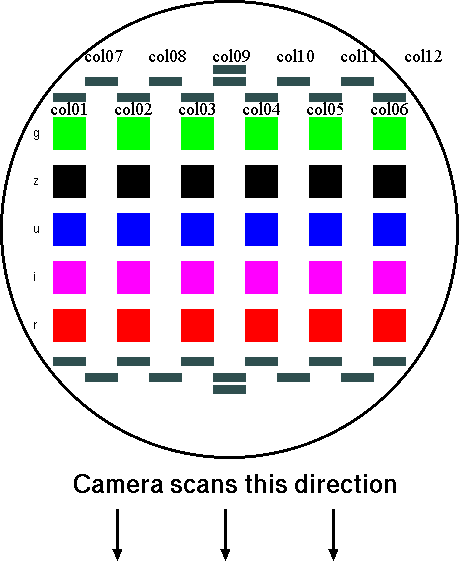
\includegraphics[width=4in]{Figures/sdss_camera.png}}
\caption{The camera used for imaging. It consists of 30 photometric CCDs, that are arranged in 6 columns of 5 each. Camera is drifted in the way that each column has permanent Declination during the run and all 5 filters in a column consequently go over the same field}
\label{fig:sdss}
\end{figure}

\subsection{Stripe 82}
Single-pass images are shallow (magnitude limit in r-band is 22.2 AB) and is not suitable for our purposes. For that reason we shall use Stripe 82, a $\approx300$ sq.degree area on the Celestial Equator in the South Galactic Cap in the Fall \citep{Adelman-McCarthy2007}. Stripe 82 is a deep survey stripe that spans $20h < RA < 4h$ and $-1.26 < Dec < 1.26$. This area was repeatedly used for calibration purposes and was scanned 70-90 times depending on RA. The advantage of these multiepoch images was quickly anticipated by various teams who stacked it and created co-added images. Annis et al. \citep{Annis2014} produced the first version of stacked images. They combined images available by December, 2005 (20-35 runs) and achieved magnitude limit 1-2 mag deeper then single-epoch SDSS products. results were published in SDSS Data Release 7 (DR7). Several teams produced their own co-adds using different strategy for the selection and post-processing of images (e.g. Huff et al.2014 \citep{2014MNRAS.440.1296H}, Jiang et al. 2009 \citep{2009AJ....138..305J}). It is important to outline that images were taken under different photometric conditions (e.g. significant moonlight and poor seeing in several runs performed in 2005-2007) and thus certain selection of the images has to be performed.

Jiang et al. 2014 (J14) \citep{Jiang2014} released a new version of co-adds in which only images that had been taken under perfect photometric conditions were used. These co-adds, that we shall use in our work are in general 0.2 mag deeper than in Annis et al. and 2 mag deeper than single-epoch SDSS images (see fig 7 in J14) and reach $5\sigma$ detection limit of 23.9, 25.1, 24.6, 24.1, and 22.8 AB magnitudes in bands u-, g-, r-, i- and z- respectively. 

\subsection{Structure of SDSS Stripe 82 files}

	We use description from J14 to present the structure of optical data. An SDSS run (strip) consists of six parallel scanlines, identified by camera columns (Figure~\ref{fig:sdss}). The scanlines are 13.5 arcmin wide, with gaps of roughly the same width, so two interleaving strips make a stripe. That creates the following sequence of columns in the direction of increasing declination:
$col01 \rightarrow col07 \rightarrow col02 \rightarrow col08 \rightarrow col03 \rightarrow col09 \rightarrow col04 \rightarrow col10 \rightarrow col05 \rightarrow col11 \rightarrow col06 \rightarrow col12$.

%\begin{figure}[!ht]
%\includegraphics[width=6in]{THE ONE THAT HAOJING SENT ME}
%\caption{sample text}
%\label{fig:sdss_s82}
%\end{figure}

The size of each SDSS image is 1489 x 2048 pixels, or roughly 9.8' x 13.5' (RA x Dec), with a pixel size of 0.396" and an average full width at half maximum (FWHM) of $\sim1.5"$ in u-band, $\sim1.3"$ in g-band, and $\sim1"$ in r-, i-, and z-bands. In total there are 401 SDSS images in each column and overall $12 \cdot 401 \cdot 5 = 24,060$ SDSS images. Between any two adjacent images there is an overlap region with a width of 128 pixels along the scan direction. Catalogs that we produce will have duplicate sources for such regions and it shall be removed in the post-processing stage by internal matching of all sources in the final catalog using the matching radius of 1.2". This radius was determined empirically to be the largest at which we do not have false rejections - rejection of two sources that lay very close to each other on the line of sight.\\ 
Images are named by their band, column and sequential number, e.g. $S82\_11x\_222.fits$, where 11 is the column number, x - letter for one of the five bands, and 222 - sequential number. Each SDSS image has a corresponding weight.fits image, that records relative weights at individual pixels.

\section{WISE}

WISE \citep{Wright2010} is a near-IR space observatory that was launched in December 2009 and mapped the entire sky with sensitivity far better than that of its predecessors, IRAS \citep{Neugebauer1984} and DIRBE \citep{Silverberg1993}. With a 0.4 m telescope on board always pointing at 90 degrees solar elongation, WISE made successful scans of the entire sky in four bands, namely w1 ($3.4 \mu m$), w2 ($4.6 \mu m$), w3 ($12 \mu m$) and w4 ($22 \mu m$). Its observations have very wide range of applications from search of near-Earth asteroids and brown dwarfs to the studies of the most luminous galaxies in the Universe.

\subsection{unWISE}

WISE data are published as a set of co-added data. Stacks were created by the WISE/NEOWISE team using the first 13 months of data (AllWISE release) and are available at NASA/IPAC \fnurl{Infrared Science Archive}{http://irsa.ipac.caltech.edu}. Original images were intentionally blurred by the WISE point spread function (PSF) for better detection of deep single sources. But that leads to the blending problem in the crowded fields and also decreases the signal-to-noise ratio (SNR) due to the broadening of the PSF. D.Lang \citep{Lang2014e} (D14) has produced custom “unWISE” stacks analogous to the AllWISE images, but at the full spatial resolution of the instrument - 2.75"/pixel. Example of the WISE team stacks and deconvolved unWISE stacks can be seen at Figure 2 in D14. unWISE images are appropriate for photometry in the crowded fields and they preserve the available signal-to-noise and we shall use it with SDSS Stripe 82 data in this project.

\subsection{Structure of unWISE files}

Structure and naming convention of unWISE files is taken from \fnurl{unwise.me}{http://unwise.me/data}. The unWISE coadds are on the same tile centers as the WISE images: 18,240 tiles per band, 1.56 x 1.56 degrees each. The tiles are named by their RA, Dec center: tile "0591p530" is at RA = 59.1, Dec = +53.0 degrees; i.e., the first four digits of the tile name is $int(RA \cdot 10)$, then "p" for +Dec and "m" for -Dec, then three digits of $int(abs(Dec)\cdot 10)$. For each tile and band w1-w4, several images are produced, we shall list only the ones that we make use of:

-- unwise-0000p000-w1-img-m.fits - "Masked" image, 2048 x 2048 pixels, TAN projected at 2.75"/pixel. Background-subtracted, in units of "Vega nanomaggies" per pixel: $mag = -2.5 \cdot (log_{10}(flux) - 9)$. This is our science image. The word "masked" means that some pixels will have no unmasked pixels and no measurement at all: pixel value 0 and infinite uncertainty.

-- unwise-0000p000-w1-std-m.fits - Sample standard deviation (scatter) of the individual-exposure pixels  contributing to this coadd pixel. This will be large if, for example, the source is variable.\\

One unWISE FITS image may cover up to 72 SDSS images within its footprint. We shall call one unWISE image or a set of SDSS images within this area "a frame".

For each coordinate in RA there are 3 unWISE images that covers all 12 SDSS columns (ranging from -1.26 < Dec < +1.26). We call such a set of three unWISE images a frame. One frame fits up to 72 SDSS images. Two adjacent frames overlap by $\sim2.9'$ and sources that appear in such regions will be duplicated. Such sources, as in the case of the overlapping SDSS images, shall be removed in the post-processing stage.



\chapter{Construction of the multiband catalog over Stripe 82}\label{CH_02}

	SED fitting requires supplying catalogs that contains multi-wavelength photometry. Quality of photometric data is very important for proper estimation of the properties of the galaxies. In this chapter we shall describe our strategy for construction of such catalogs, optical and IR, general issues that arise and our methods to solve it.
	
	SDSS co-adds from J14 that we utilize already have catalogs on the whole Stripe 82 region. We decide not to use it and create our own catalogs for several reasons:\\
	-	The catalogs are not matched between the bands, resulting in different object lists for each band within the same region,so there may be misidentification of the sources when we attempt to construct multiband catalog with data from all 5 bands.\\
	-	SNR at which the source is rejected from the catalog was chosen too high and there are a lot of sources that we shall use, which are not included in J14 catalog.\\
	-	Bright and saturated objects are generally represented in this catalog as multiple sources, none of which is at the center of such object. This means that when SED fitting is performed for this source, non-physical stellar mass and redshifts will be produced. \\
	On Figure~\ref{fig:catalog_comp} we present a comparison of the original catalog from J14 (sources within green regions) and our catalog, that was constructed independently (sources within red regions) and will be presented further in this chapter.
	
\begin{figure}[!ht]
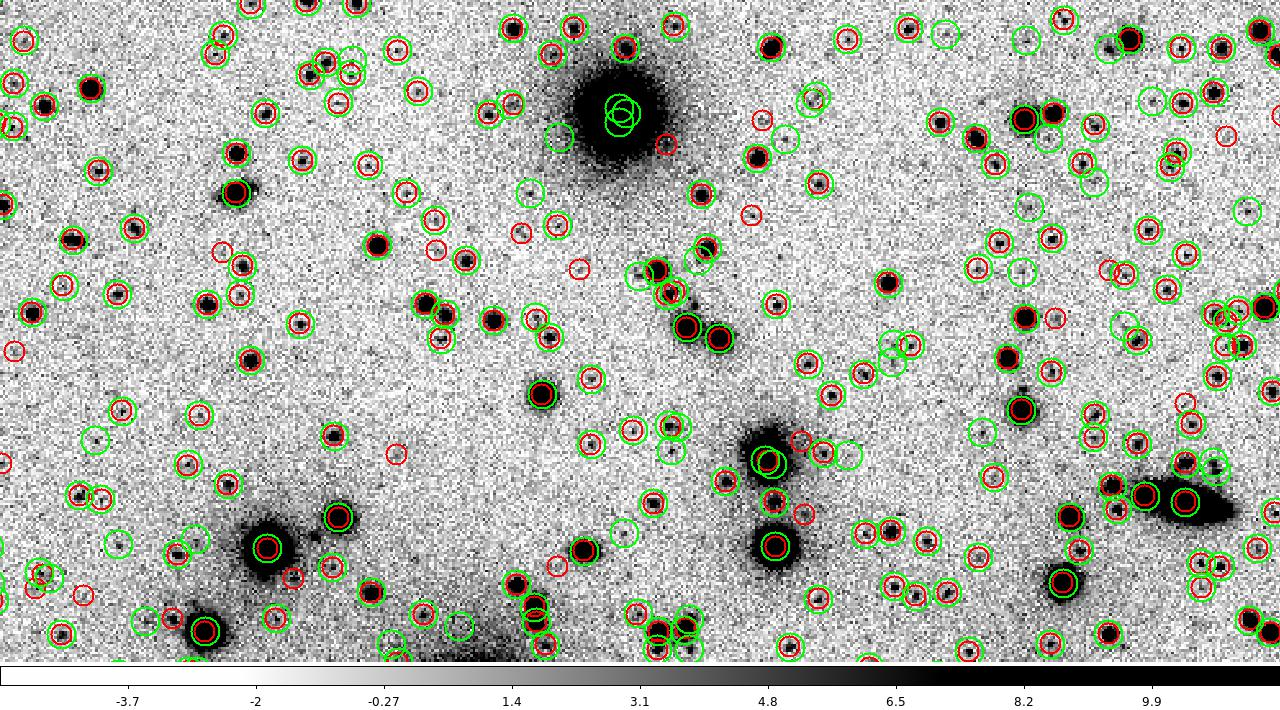
\includegraphics[width=6in]{Figures/catalog_comparison.jpeg}
\caption{Optical catalogs from J14 (green circles) and our catalog (red circles) are overplotted on a small random area in Stripe 82. There is a number of well-detected sources that were excluded from J14 catalog and also there are multiple detections around a saturated source in the upper part of the plot. Our catalog aims to resolve both such issues.}
\label{fig:catalog_comp}
\end{figure}	
	
	
	The most critical factor in the success of this project is consistent photometry from optical to near-IR. This is challenging because the spatial resolutions of WISE is $\sim$5-6x worse than that of SDSS. For this reason, the objects detected in WISE often suffer blending. Even for relatively isolated WISE sources, the photometric apertures appropriate for the (low resolution) WISE images cannot guarantee the same fraction of light being included as what is done in the (high resolution) SDSS images. Such a systematic offset, which is different for every galaxy of different morphology, can severely skew the SED fitting.

To best address this problem, we opt to use the {\tt TPHOT} software \citep{Merlin2016a}, which recently emerged as a robust and flexible tool to perform $"$template fitting$"$. The basic idea is to use a high-resolution image (here SDSS) as the prior to build the morphological template of the source under question, convolve this template with the PSF of the low-resolution image (here WISE), and fit this degraded template to the low-resolution image to obtain the total flux that is within the aperture as defined by the high-resolution image. In this way, we get reliable color information (i.e., flux ratio) in the most consistent manner. It is important to note that high-resolution source does not have to be point-like - its morphological features will be preserved and fitted to the low-resolution source. This implies the biggest assumption for this technique - that morphology of the source is wavelength-independent. While generally it is not true, especially for the actively star-forming or dusty galaxies, we anticipate that this will not create any significant bias. Firstly, because most of the galaxies have small angular sizes and such variation in sizes is small (galaxy at z=0.7 that is 40 kpc in diameter has an angular size of only 6 pixels), and secondly, because we chose SDSS r-band ($6202.46~\AA$), that is a red filter, as a high-resolution image - there should not be much morphological difference between r-band and w1 or w2 bands..\\

Proper use of {\tt TPHOT} requires several preliminary operations with both high- and low-resolution images, and construction of optical catalogs also consists of a number of steps. It is impossible to separate operations for these two main stages - chronologically the steps for both stages are intermixed. In the following sections we shall describe general algorithm in the order in which it was implemented in the project.

\section{Preparatory work with SDSS images and optical catalog}
	
	High-resolution optical image is used not only to determine flux and morphology of the source in near-IR, but also its position. For that reason high- and low-resolution images should have the same type of projection, reference coordinate and orientation written in their FITS headers \citep{Pence2010}. SDSS and WISE images have the same tangential projection and orientation ($CD1\_2=0$, $CD2\_1=0$), so we leave these values unchanged. Each WISE frame covers $\approx 3.95 deg^{2}$ and there may be up to 72 SDSS images that cover the same area, so we decide to use coordinates of the center of WISE images (CRVAL1 and CRVAL2) as the anchor values and run {\tt SWarp} \citep{Bertin2002} to change reference pixels in all SDSS images. The reference pixel (CRPIX1 and CRPIX2) for SDSS images can now be outside of the image itself to as far as 0.7 deg. 
	
\subsection{Region of overlapping unWISE images}

Some SDSS images may reside on the border between two overlapping unWISE images. In such a case 2 copies of SDSS image are created, each is processed by {\tt SWarp} independently, gets its own set of CRPIX and CRVAL values and from now on is treated separately. 
The following example shows the current naming convention that is used throughout this work: $S82\_3282m016\_01r\_097.fits$ and $S82\_3297m016\_01r\_097.fits$ means that original image $S82\_01r\_097.fits$ now has two sets of CRVAL values - one is the same as the coordinates of the center of image unwise-3282m016-w1-img-m.fits and the other - of image unwise-3297m016-w1-img-m.fits.

This "duplication" increased the number of SDSS images in each band from 4,812 to 5,556.
	
\subsection{SDSS PSF construction}
	Optical part of the catalog consists of 5 SDSS bands, each of which has different sensitivity and FWHM, so each field has different number of sources in different bands. We shall choose the band that we use for detection, i.e., the source is added to our catalog if only it is detected in this band with sufficient SNR. Also position of the source in this band is used as the true position in all other bands. Another issue is the flux measurement - reliable SED fitting requires consistent multiwavelength photometry while different photometric conditions and FWHM could result in a non-consistent colors even in optical filters alone. Thus the measurment that are made even with flexible elliptical apertures known as the Kron apertures \citep{Kron1980} that are denoted  in {\tt SExtractor} as FLUX\_AUTO \citep{Bertin1996} will not be measuring the same fraction of the total flux from the given source in different filters. We decided to convolve \textit{griz} bands to the one with the worst FWHM, i.e., u-band. In such case the difference in sizes will be due to the intrinsic difference in morphology at different wavelength rather than due to difference in optics. For the price of loosing some sources due to blending we shall achieve better consistency in our optical colors. We use {\tt IRAF/psfmatch} task that requires supplying the image with the corresponding kernel - PSF matching function to be convolved with the input image to produce the output one. Construction of a kernel requires a knowledge of the PSFs of the input image and a matched image. That means we need to construct PSF for each image in each band ($5,556\cdot 5 = 27,780$ PSFs) and this is the most time-consuming part of the project.

One of the widely-used ways to construct a PSF is using {\tt PSFEx} software \citep{Bertin2011}. We tested it with {\tt TPHOT} and found that the quality of residual images is not satisfactory, so we decided to use more conservative algorithm in which {\tt IRAF/psf} task creates a PSF function based on a set of selected point-like sources (so called PSF stars). Usually that strategy involves consecutive run of {\tt IRAF/find}, {\tt IRAF/phot}, {\tt IRAF/pstselect} and {\tt IRAF/psf} tasks that find stars, determine its magnitude, select the ones that do not have any morphological features and finally construct a PSF function. This algorithm, though much more reliable, is also not ideal - in each image there are $\sim 10\% $ of sources that do not satisfy the criteria of PSF stars (are elongated, blended or have noisy background) and have to be rejected in the manual regime (selection in interactive mode). This is extremely time-consuming and inefficient given the total number of images in 5 bands. We decide to use a variation of this method to create PSF functions in a more automatic fashion that is presented in the next passage. 

We run {\tt SExtractor} on each SDSS image and only mark sources from the output catalog as a point-like, if their "stellarity" index (determined by a CLASS\_STAR parameter) is close to 1, sources are bright, but not saturated, do not lay within $2 \cdot PSF~radius$ to the edge of the FITS image, and have all their flux contained within some small aperture. The later was confirmed by finding the difference "MAG diff" between MAG\_APER that returns all flux within some fixed aperture and MAG\_BEST that returns MAG\_AUTO value in the absence of contamination from the nearby sources and MAG\_ISOCOR otherwise. Exact parameters depend on the band and also were adjusted during test runs so that each SDSS image has no less than 20 PSF stars (stars were sorted by their magnitude, from bright to dim), with the maximum number of PSF stars limited to 160 (larger values significantly slow down {\tt IRAF}). Selection criteria can be found in Table~\ref{tab:psf_star}

\begin{table}[h!]
  \begin{center}
    \caption{Table of parameters for selection of PSF stars}
    \label{tab:psf_star}
    \begin{tabular}{l|l|l|l|l|l} % <-- Changed to S here.
      \textbf{parameter} & \textbf{u} & \textbf{g} & \textbf{r} & \textbf{i} & \textbf{z}\\
%      $\alpha$ & $\beta$ & $\gamma$ \\
      \hline
%      aperture [pix]  & ?? & ?? & ?? & ?? & ??\\
      MAG diff & -0.06 -- -0.14 & -0.04 -- -0.1 & -0.1 -- 0.7 & -0.1 -- 0.7 & -0.1 -- 0.7\\
      CLASS\_STAR min & 0.80 & 0.85 & 0.85 & 0.85 & 0.80\\
      MAG\_AUTO min   & 13.5 & 13.8 & 14.2 & 13.7 & 13.1\\
      MAG\_AUTO max   & 19.0 & 19.3 & 19.2 & 19.1 & 19.0\\
    \end{tabular}
  \end{center}
\end{table}

Selected PSF stars were supplied to {\tt IRAF/psf} to create PSF files. This task was run in a non-interactive (automatic) mode with parameters listed in Table~\ref{tab:table2}

\begin{table}[h!]
  \begin{center}
    \caption{Table of parameters for {\tt IRAF/psf} task.}
    \label{tab:table2}
    \begin{tabular}{l|l|l|l|l|l} % <-- Changed to S here.
      \textbf{parameter} & \textbf{u} & \textbf{g} & \textbf{r} & \textbf{i} & \textbf{z}\\
      \hline
      fitrad & 2.9 & 2.8 & 2.7 & 2.7 & 2.8\\
      fwhmpsf & 2.9 & 2.8 & 2.65 & 2.65 & 2.8\\
      sigma & 0.48 & 0.70 & 0.65 & 0.48 & 0.77\\
    \end{tabular}
  \end{center}
\end{table}

Parameters that were the same for all bands:\\
\begin{tt}
functio=             moffat25\\
matchra=                   3\\
psfrad =                  12\\
nclean =                    3\\
noise  =              poisson\\
	\end{tt}

After we obtain all PSF functions for our sample, we run {\tt IRAF/seepsf}, a task that takes the input PSF computed by the {\tt IRAF/psf} task, consisting of the parameters of a 2D analytic function stored in the image header, and computes 21x21 pixel output PSF FITS image consisting of the sum of the analytic function and the residuals. Visual inspection of all PSF images revealed a certain fraction of defect PSFs. The reason for it can be either a blended source within the PSF radius, high background values due to the nearby bright star (within up to several arcmin), or noticeable elongation of the source (may be due to inclusion of a galaxy in our sample or due to intrinsic problems with SDSS image).

The fraction of such images varied in different bands but generally was $\sim 4\%$ and for such images we re-run {\tt IRAF/psf} in interactive mode (manually selecting PSF stars from a catalog). All PSF images were scaled to unit flux using {\tt wcstools/sumpix} \citep{Mink1998b} and {\tt IRAF/imarith} tasks. Several PSFs for all 5 bands and 6 different columns centered at RA=21:56:46 are shown in Figure~\ref{fig:psf}

\begin{figure}[!ht]
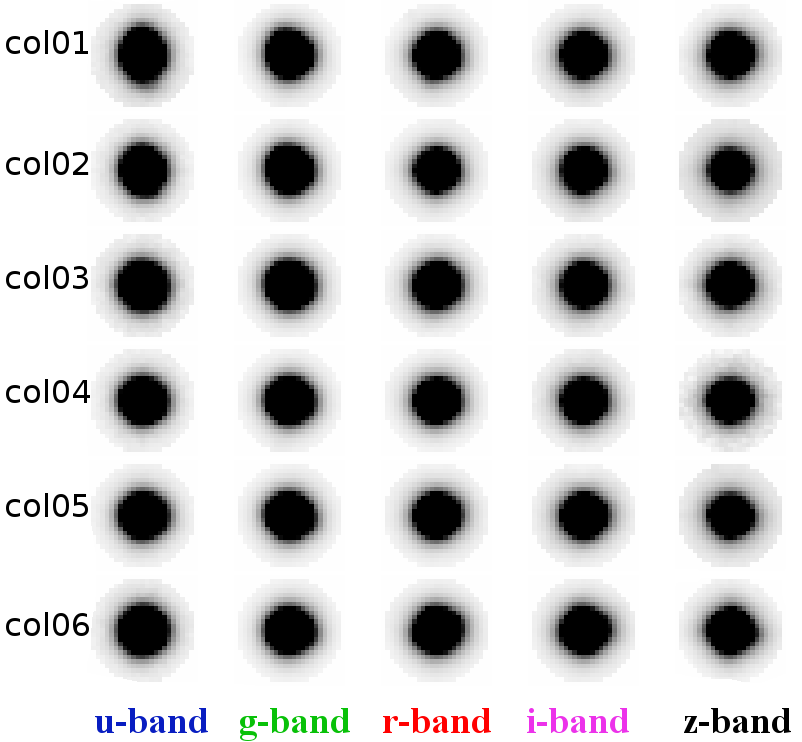
\includegraphics[width=6in]{Figures/psf_allbands_6cols.png}
\caption{A set of PSFs for five bands for odd columns centered at RA=21:56:46. All PSFs are scaled to the unit flux}
\label{fig:psf}
\end{figure}

We used {\tt IRAF/lucy}, a task that uses algorithm developed independently by Lucy \citep{Lucy1974} and Richardson \citep{Richardson1972}, to create kernels for pairs of images in x- and u-bands, where "x-" stands for g-, r-, i-, or z-band. 
Parameters  for {\tt IRAF/lucy} :\\
\begin{tt}
input  = u-band PSF\\ 
psf    = g-, r-, i-, or z-band PSF\\ 
niter  =  50\\ 
limchis=  $1.0E-14$\\ 
accel\_m=  standard\\ 
	\end{tt}

With kernels in hand it is now possible to run {\tt IRAF/psfmatch} that convolves input image with the kernel to produce a psf matched output image (Figure~\ref{fig:psfmatch}). 
Parameters  for {\tt IRAF/psfmatch} :\\
\begin{tt}
input = g-, r-, i-, or z-band FITS  file\\ 
kernel = kernel.fits\\ 
output = x\_matched\_u.fits\\ 
convolu = kernel\\ 
	\end{tt}

\begin{figure}[!ht]
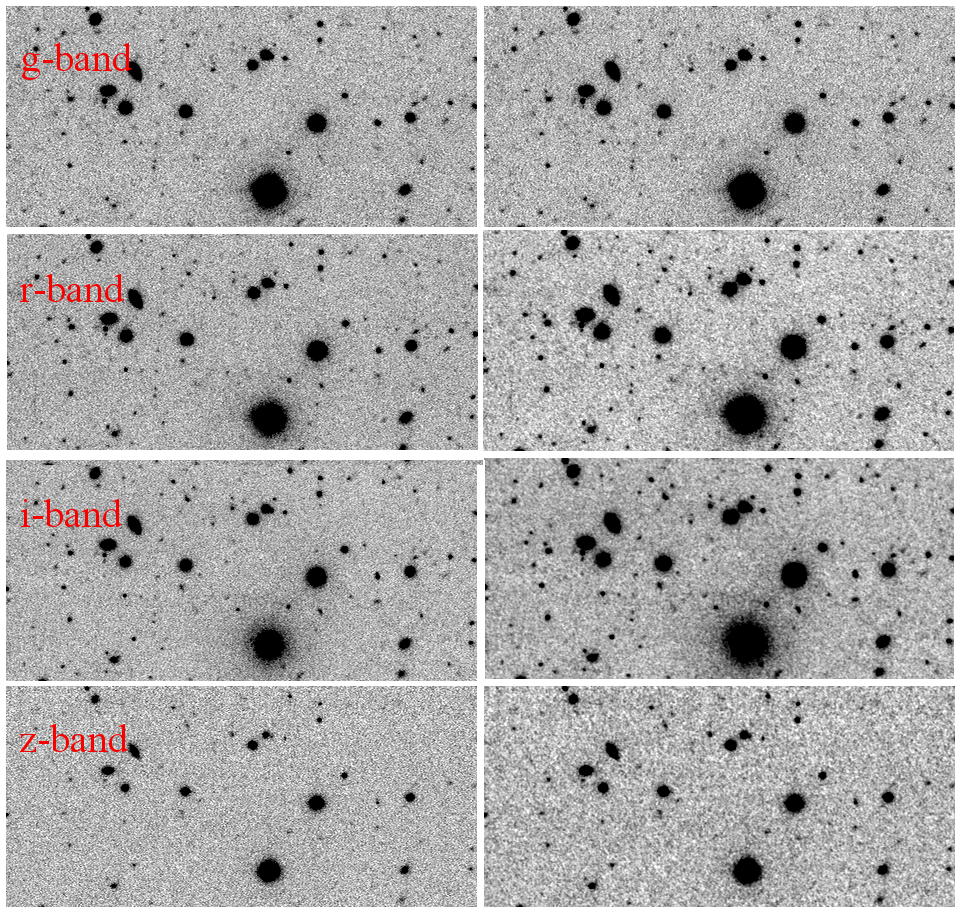
\includegraphics[width=6in]{Figures/psfmatch.png}
\caption{An example of {\tt IRAF/psfmatch} for $griz$ bands (top to bottom). Original images are to the left, PSF-matched - to the right. The difference is mostly observable for r- and i-bands, because their  PSF is much better than that of the u-band}
\label{fig:psfmatch}
\end{figure}


\subsection{Construction of the optical part of the catalog}
As outlined above, different bands have different sensitivity and FWHM, so faint sources may not be detected in all bands. In order to construct our catalogs we ought to select one band as the detection band. It has to be deep enough to have as many sources as possible and also has good FWHM to constrain the shape of the sources - that is crucial for the flux measurement in unWISE bands as each image must be supplied to {\tt TPHOT} along with the corresponding segmentation file and also each source in the catalog must have its x\_min, x\_max, y\_min and y\_max vales. As can be seen on Fig.9 from J14, $riz$ bands have the best FWHM out of 5 bands, and among them r-band has the highest limiting magnitude (24.6, comparing to 24.1 and 22.8 AB magnitudes in i- and z-band respectively). We choose r-band to be the base catalog of our sample and we used position of the source in this band to extract flux in $ugiz$ bands in SDSS and also in w1 and w2 bands of unWISE images.

Now we run {\tt SExtractor} in the dual mode (the first image is used for detection and astrometry information, while the second is used solely for photometry) to create a 5-band optical catalog. We use r\_matched\_u images for the detection of sources and x\_matched\_u image for the photometry, (u\_matched\_u is just u-band image). All bands are PSF matched to the u-band, and thus the same FWHM so {\tt SExtractor} parameters are identical with the exception of the magnitude zeropoint. Complete list of parameters is provided in \hyperref[sec:sex]{Appendix}. As the next step we reject sources with SNR $<5$ based on the r\_matched\_u flux. We notice that very few sources were rejected at this stage - objects that appear almost undetectable had FLUX\_AUTO / FLUXERR\_AUTO larger than 5 or even 7. We address this issue in the next section, and note that we decide not to reject those sources and supply it to {\tt TPHOT} because we shall use residual images to detect "WoDrops" - objects that are undetectable in optical bands. i.e., dropouts. But for the purpose of the GSMD construction we corrected magnitude errors and rejected sources with SNR $<5$ before starting the SED fitting.

\subsection{Magnitude error correction}

Photometry comparison between original x-band and x$\_$matched$\_$u-band catalogs shows a systematic underestimation of the errors associated with the sources' flux (Figure~\ref{fig:err_corr}). To correct for that we use {\tt STILTS} code \citep{Taylor2006} to match x-band and x$\_$matched$\_$u catalogs in 5 bands and for each separate image we calculate the mean ratio of the flux error before and after PSF. 
All magnitude errors in a given image are then multiplied by this coefficient. This correction coefficient can also be used as a test of our PSFs - all coefficients should occupy a narrow region with values within 1.2-2.2 for $griz$ bands with very few outliers (Figure~\ref{fig:err_corr_coef}).
We did not apply {\tt IRAF/psfmatch} task to the u-band, but still calculated that correcting coefficient because r\_matched\_u FITS file was used as detection image in {\tt SExtractor}. All coefficients for this band are less than 1. 

\begin{figure}[!ht]
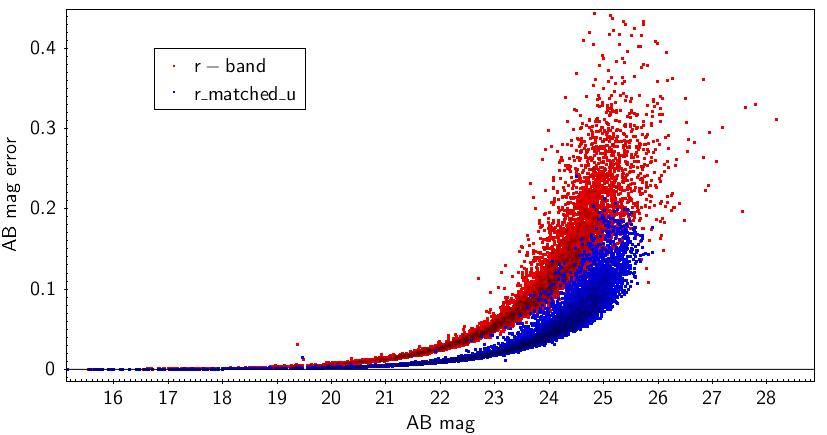
\includegraphics[width=6in]{Figures/error_correction_rband_example.jpg}
\caption{An example of the change in magnitude error for r-band photometry. Original errors are plotted against AB mag in red, magnitude errors \textit{for the same source} after {\tt IRAF/psfmatch} is performed are in blue.}
\label{fig:err_corr}
\end{figure}

\begin{figure}[!ht]
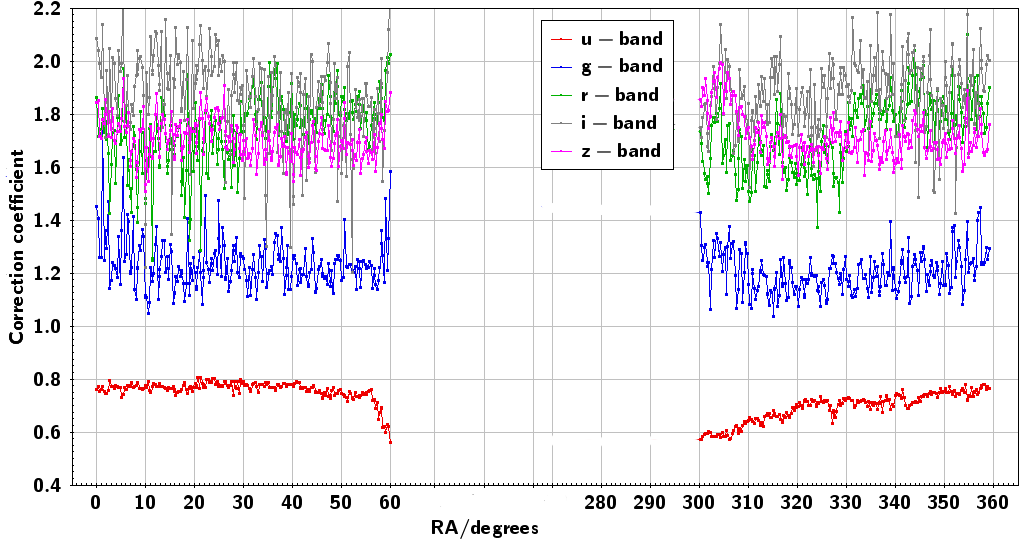
\includegraphics[width=6in]{Figures/magerr_corr_04.png}
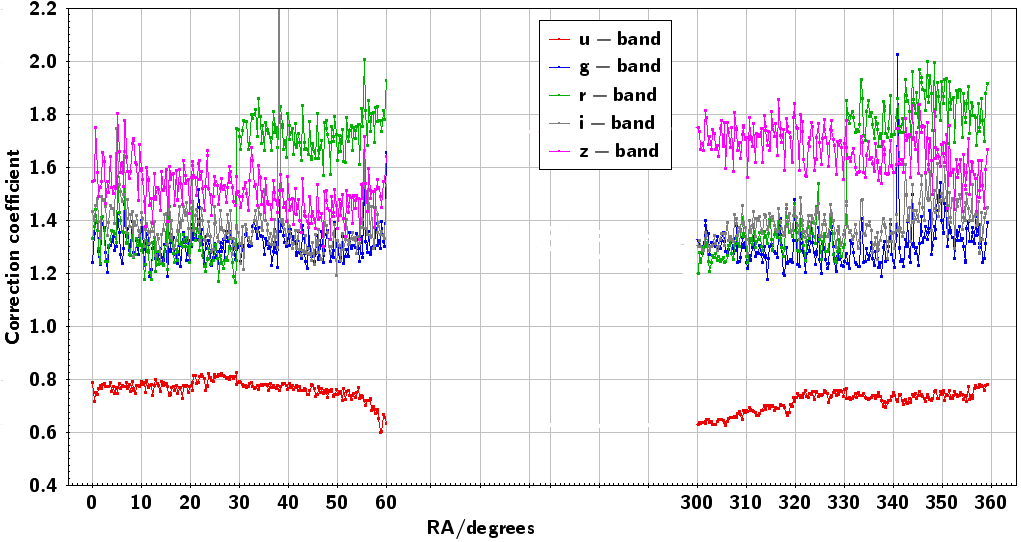
\includegraphics[width=6in]{Figures/magerr_corr_12.png}
\caption{Correction coefficients for all 5 bands for two columns - col04 (top) and col12 (bottom). Note that coefficients for the u-band are less than one}
\label{fig:err_corr_coef}
\end{figure}

We anticipate that while corrected values account for statistical error, there should also be a systematic error in magnitude that needs to be taken care of. We performed a series of tests where different constant errors were added in quadrature to the reported magnitude error and then the goodness of fit on the graph z\_spec vs z\_phot was checked. We found that correlation is the tightest when 0.04 magnitude error is added in quadrature (so final error cannot be smaller than 0.04). So finally, each source in each band was assigned by a error in magnitude that was calculated using the following equation: 
$$ magerr\_corrected = \sqrt{0.04^{2}+(\dfrac{1.0857}{SNR}\cdot correction\_coefficient)^{2}}$$

At this point construction of the optical part of the sample is complete. Our parent catalog now consists of 26,585,000 sources. 

\section{Preparatory work with unWISE files}
	{\tt TPHOT} is very demanding to the quality of the input files, any small variation severely skews results, so we pay particular attention to this part.
	
\subsection{unWISE PSF construction}
	
We use {\tt SWarp} to change the pixel scale of all unWISE images from original 2.75 to 2.772 to match the integer pixel scale ratio with SDSS images $\dfrac{2.772}{0.396}=7$. Now we construct unWISE PSF functions that is to be convolved with SDSS PSF to produce kernels - one of the most important set of the input files to {\tt TPHOT}. There are 240 unWISE images within Stripe 82 footprint per band. Bands w3 and w4 are too shallow and no reasonable flux can be extracted for the vast majority of optical sources  in these bands, so for the purpose of this project we only use w1 and w2 bands. That means we need to make another 480 PSFs.
We followed the strategy from the previous section to construct PSF for all 480 images (i.e., running {\tt SExtractor}, selecting potential PSF stars using {\tt STILTS}) with two major differences in the procedure:\\
1) Center pixels of saturated sources in unWISE standard deviation images (unwise-0000p000-w1-std-m.fits) always have zero value and that is an invalid input for {\tt TPHOT}. We use {\tt IRAF/imcalc} to detect such pixels and change its value to "9999".\\
2) We construct each PSF function manually, using {\tt IRAF/psf} in interactive mode. This was done to perform more robust selection of stars as 3 PSFs from one unWISE frame are convolved with 72 SDSS PSFs and thus its quality is crucial - incorrect PSF profile leads to wrong flux estimation associated with such sources and also characteristic positive and negative ring-shaped patterns in the residuals. \\
After running the {\tt IRAF/seepsf} task we get PSF FITS images, 19x19 pixels each. All unWISE PSFs are then scaled to the unit flux with {\tt IRAF/imarith} and sub-sampled in size by the factor of 7 using {\tt IRAF/imlintran} (to 133x133 pixels) to match the pixel scale ratio between unWISE and SDSS images. Result is presented on Figure~\ref{fig:unwise_psf}

\begin{figure}[!ht]
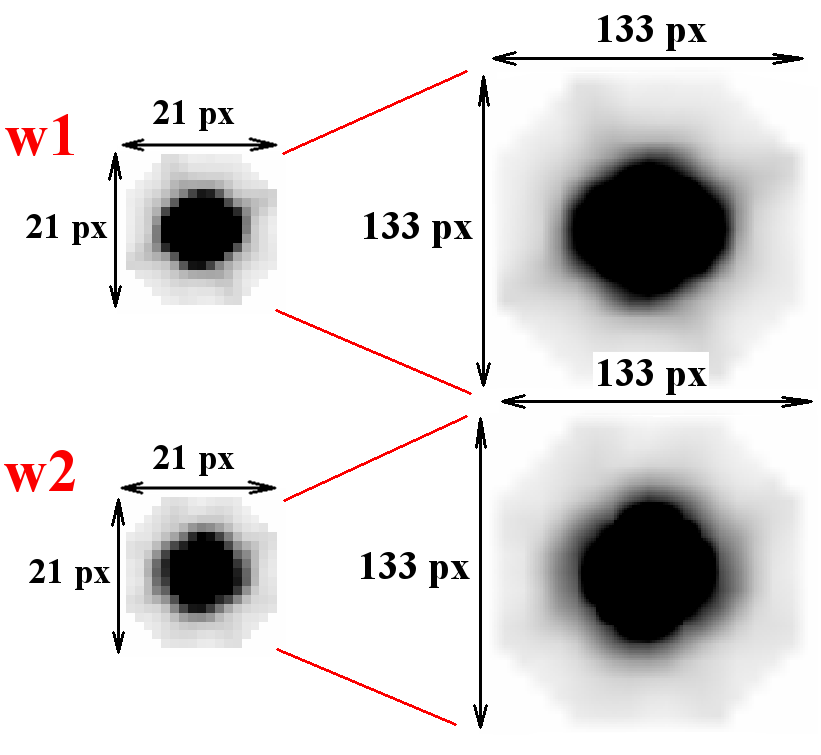
\includegraphics[width=6in]{Figures/unwise_psf.png}
\caption{unWISE PSFs for w1 (top row) and w2 bands (bottom row), as constructed in {\tt IRAF/psf} (left) and scaled by factor x7 to mimic pixel scale ratio between SDSS and unWISE pixel scales (right)}
\label{fig:unwise_psf}
\end{figure}

\subsection{Naming convention for the processed files}

Both final and intermediate results are a combination of SDSS and unWISE data and we introduce our naming convention that is used throughout the project. E.g. file
kernel.w1.0000p015\_12r\_u\_111.fits is a kernel made by convolution of the PSF function of the file unwise-0000p015-w1-img-m.fits and PSF function of the file S82\_12r\_111.fits in r-band, that has been previously matched to the PSF of the u-band.


\section{Template fitting with {\tt TPHOT}}
{\tt TPHOT} is a software designed to perform a precision photometry on a low-resolution images using information provided by a high-resolution images of the same field. Running {\tt TPHOT} on such a large portion of the sky with individual kernels for every pair of high- and low-resolution image is a key feature of our project.

In order to get the best results we follow recommendations of E.Merlin and perform two runs ("pass 1" and "pass 2") of {\tt TPHOT} on each pair (low- and high-resolution) of images. The second pass is performed using local kernels registered after the shifts in x and y coordinates are determined in the first pass.

One of the advantages of {\tt TPHOT} is a large saving of computational time comparing to its forerunners, {\tt TFIT} or {\tt CONVPHOT} codes, but it still needs lots of CPU time. Each SDSS image has on average 5200 sources and each pass of {\tt TPHOT} takes $\sim3$ hours CPU time. We perform template fitting on two unWISE bands so the total number of passes is $5556 \cdot 2 \cdot 2$ that requires $\approx 66,700$ CPU hours. We use our access to the University of Missouri High-Performance Computing (HPC) cluster ”Lewis” to process all images.

There are six different files supplied as an input to each run of {\tt TPHOT}:\\
-	High-resolution image - SDSS r-band FITS image matched to the u-band PSF\\
-	Source catalog with position, flux and background measurements for each source\\
-	Segmentation map corresponding to the SDSS image and having the value of the id of each source in the pixels belonging to it, and zero everywhere else\\
-	Low-resolution image - unWISE either w1 or w2 FITS image\\
-	Low-resolution weight image\\
-	kernel - result of convolution of high- and low-resolution PSFs\\

Dimensions of high- and low-resolution images do not have to be the same for successful run of {\tt TPHOT}, so generally we can supply full unWISE frame as the low-resolution image, but the code performs certain mathematical operations on such image during each pass, and such operations are mutually interfering when one tries to simultaneously run {\tt TPHOT} on several SDSS images that belong to the same unWISE frame. In order to run several {\tt TPHOT} jobs at the same time at Lewis cluster we created 18.828'x13.523' unWISE cutouts (with associated weight image) for each SDSS image.

After considerable number of test runs we came up to the following set of parameters that provides us with the best results. We only list the most important parameters here, full list is available in \hyperref[sec:tphot]{Appendix}:\\
{\tt order standard 			}$\#$ Used for the first pass\\
{\tt order standard2 		}$\#$ Used for the second pass\\
{\tt usereal         True    }$\#$ Real 2-d profiles\\
{\tt relscale        7		}$\#$ Pixel ratio between detection and measure image\\
{\tt FFTconv         true 	}$\#$ Use FFT for convolution of cutouts\\
{\tt fitting         single	}$\#$ One of three possible fitting methods\\
{\tt fitbackground   false}\\
{\tt clip            true 	}$\#$ Clip out large negative fluxes and re-do the fit\\
{\tt dzonesize       5 		}$\#$ Pixels size of region in which PSF shift is computed\\

\subsection{{\tt TPHOT} output files}

The most important {\tt TPHOT} output files are low-resolution residual FITS image, which is obtained by subtracting the model image from the low-resolution image, and catalog of residual fluxes and corresponding flux errors for each input source that was successfully fitted. {\tt TPHOT} rejects source if it lies outside of the low-resolution frame or if it has too high RMS. For such rejected source the fitted flux and flux errors are assigned to be $-99$ and $99.0E8$ respectively - such source is still used for SED fitting and we do not create any special subsample for the sources without near-IR photometry. On Figure~\ref{fig:resid} three images are shown - r-band SDSS, w1-band unWISE and residual in w1-band. Red circles with 3" radius are drawn around optical sources that are supplied to {\tt TPHOT}.

\begin{figure}[!ht]
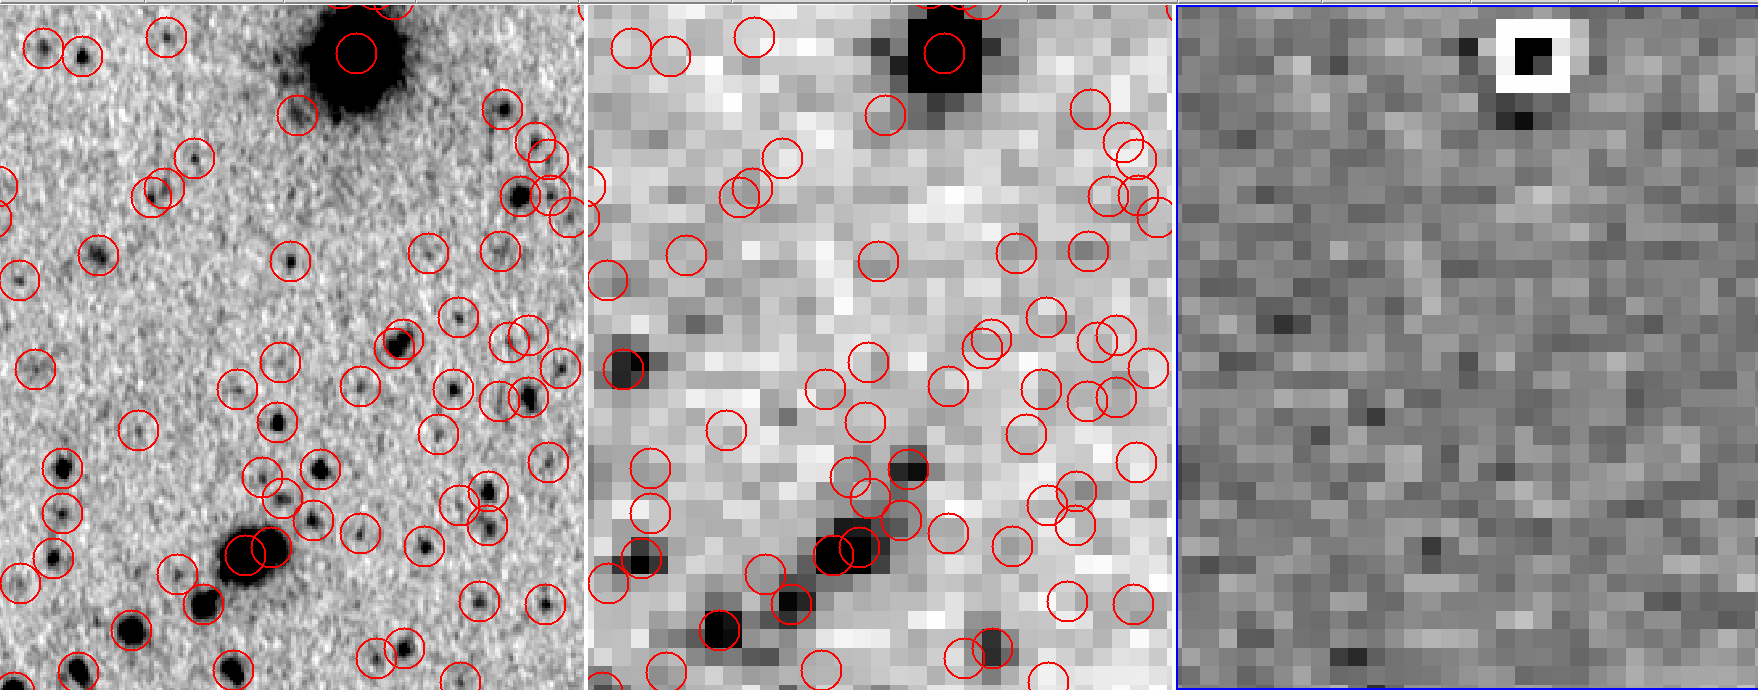
\includegraphics[width=6in]{Figures/sdss_unwise_resid.png}
\caption{From left to right: SDSS image in r-band, unWSIE w1 image, residual image from {\tt TPHOT}. SDSS sources that are fitted to the unWISE image for the flux estimation are denoted with red circles. These objects are cleaned out from the residual image}
\label{fig:resid}
\end{figure}


\section{Matching optical and IR catalogs}

Once all unWISE images within Stripe 82 footprint in w1 and w2 bands are processed by {\tt TPHOT}, output catalogs need to be matched with optical ones. Matching is performed with {\tt STILTS} code by using the source ID as the parameter to match. Additional test is performed in order to verify that photometry in optical and IR indeed belongs to the same source: difference in r-band {\tt FLUX$\_$ISO} and {\tt TPHOT} input flux in both bands is calculated and it should be zero.

As the next step fluxes in the matched catalogs are converted from counts/sec to AB magnitudes and flux in microJansky.

\chapter{Mass and redshift estimation}\label{CH_03}

Fitting the spectral energy distributions (SEDs) of galaxies is an almost universally used technique to derive a range of physical properties of galaxies, such as redshift, stellar masses, star formation rates, dust masses, and metallicities (though there is a temptation to over-interpret the available data, so results should be taken with caution). SED fitting has matured significantly in the last decade and model predictions and fitting procedures have increased the precision of the results, attempting to keep up with the vastly increased volume and quality of available data. For this project we will use SED fitting to estimate redshift of individual galaxies and their corresponding stellar mass.

Traditionally, photometric redshift estimation is generally presented by two large groups of algorithms: empirical methods and the template-fitting methods (not to be confused with the template-fitting technique that we use to perform photometry on near-IR images). Empirical methods use a subsample of the photometric survey with spectroscopically-measured redshifts as a "training set" for the redshift estimators. This subsample describes the redshift distribution in magnitude and color space empirically and is used then for calibration of the whole sample. We list several training set based codes: ANNz \citep{2004PASP..116..345C}, RFPhotoZ \citep{2008ASPC..394..521C}, Singal \citep{2011PASP..123..615S}. Template methods use libraries of either observed spectra of galaxies exterior to the survey or template SEDs, that are built using different stellar population synthesis (SPS) models. As these spectra are produced artificially, they span over full spectra, and templates can be shifted to any redshift and then convolved with the transmission curves of the filters used in the photometric survey to create the template set for the redshift estimators. Among some most widely used template based codes we list BPZ \citep{2011ascl.soft08011B}, HYPERZ \citep{Bolzonella2011} and Kcorrect \citep{Blanton2017}. Both methods then use these training sets as bases for the redshift estimating routines, which include $\chi^{2}$-fitting and various machine learning algorithms (e.g. artificial neural networks, ANNs). A good review of the present state of the art in the area of fitting SED of galaxies is presented in \citep{Walcher2011} and a list of codes with documentation, reviews, discussions and templates is available at \fnurl{sedfitting.org}{http://www.sedfitting.org/Fitting.html}

For several years best results in SED fitting were obtained by the codes that calculate redshift based on the flux determined from the red-sequence stars - redMaPPer \citep{2014ApJ...785..104R}, redMaGiC \citep{2015MNRAS.453...38R} or that use a trained neural network (ANNz \citep{2004PASP..116..345C}). Recent studies \citep{Bundy2015} show that these codes get twice smaller scatter of z\_phot vs z\_spec for massive galaxies. But for the faint galaxies (i-band magnitude $> 22.5$ AB), template codes perform slightly better, probably because of the smaller training sets available for neural networks and obviously poorer photometry. Our catalog consists of over 23 millions of objects, and calculation speed is also an important factor for the section of the fitting code. Computationally, most template-fitting codes benchmark roughly similarly, while the training codes are much faster to evaluate the redshifts but only after their training is complete. The quality of our data was refining while the project was already ongoing and we did not attempt to use the empirical-based codes as it would have required re-computation of the training set after each change in the algorithm (e.g., we did not plan to perform matching to the u-band PSF originally). Thus we chose to test several template-fitting codes to find which one gives the best results.

\section{SED fitting}

\subsection{Choice of SED fitting codes}

A special case of analyzing SEDs of extragalactic sources
is the problem of redshift estimation, a topic that is usually
referred to as photometric redshifts (hereafter z\_phot). This
problem is different from all other estimates of physical properties (stellar mass, star-formation rate, mass of dust and gas, age) because independent and more precise measurements of the same property are available for large samples in the
form of spectroscopic redshifts (assuming some cosmological model). Results of SED fitting can thus be
tested extensively and parameters are calibrated empirically. It is also
historically one of the earliest forms of SED fitting, having been suggested as a manner to go beyond the limits of early spectroscopy \citep{1957AJ.....62....6B}.

We performed our own analysis using the first set of data that we got in the SHELA region \citep{Papovich2016}. It covers $\approx24$ $deg^{2}$ and contains over 1,800,000 sources. We do cross-matching between our catalog and SDSS DR14 release using SQL Query CasJobs. The table "SpecObj" contains data from all available SDSS spectroscopic catalogs. There are 15,790 sources in our catalog that have counterparts in SDSS DR14 within 1" and have spectroscopic redshift. We used this sample to test photometric redshifts produced by three different SED fitting codes - HYPERZ \citep{Bolzonella2011}, LePhare \citep{Arnouts2011} and EAZY \citep{Brammer2008}.

HyperZ and LePhare produced marginally the same results with the only difference that LePhare does not assign a source with the photometric redshift if the $\chi^{2}$ value is too high. Our research suggests using information from as many sources as possible and we turned down LePhare.

Tests of EAZY reveal not just the tighter correlation between spectroscopic and photometric redshifts, but also significantly smaller CPU time needed. EAZY works approximately 10 times faster and computes redshifts for a catalog that contains 50 thousands sources in 10 minutes. Considering the size of our catalog, EAZY was a natural choice for the photometric redshift determination.

We observe an unusual scatter in our data around redshift $z\approx0.4$ when comparing to the spectroscopic sample. Similar behavior can be seen in See Figure 4 in Bundy 2015 \citep{Bundy2015}, Figure 7 in Rowan-Robinson \citep{Rowan-Robinson2008} and Figure 11 in Brammer et al. \citep{Brammer2008}. SED fitting technique depends on strong features in the SEDs of the objects, such as the Balmer break, strong emission lines or even PAH features \citep{2009MNRAS.394..375N}. We try to investigate the nature of such scatter. It may not be due to the misidentification of the Lyman break as the Balmer/4000A break because we have very few galaxies with $z>1$ in our sample. Next, we examine the possibility that strong emission lines can alter the redshift. We downloaded SDSS DR14 data for certain emission lines and used flux and emission width of O[II], O[III] and Halpha lines. We compared two sets of galaxies around z=0.4 - the one with correct identification of the photometric redshift and the other that has severe offset. We did not observe any correlation between deviation of the photometric redshift from spectroscopic one and the strength of any lines.

This scatter can be slightly reduced by rejection of certain templates available for SED fitting, but there is not strict justification for choice of any particular template that is rejected, so we did not proceed in this way. We claim that such scatter in redshift determination should not affect our main results and we address this issue in the next chapter (binning).

\subsection{EAZY and FAST}

We used EAZY code to compute photometric redshifts based on optical and near-IR fluxes that we accumulated in our catalogs. EAZY \citep{Brammer2008} is photometric redshift code which was written for samples with incomplete and/or biased spectroscopic information. The code combines features from various existing programs: the possibility of fitting linear  combinations of templates (as done in GREGZ), the use of priors (as first done in BPZ), and a user-friendly interface based on HYPERZ. The default template set and the redshift-magnitude priors are derived from semi-analytic models. These models are, of course, only an approximation of reality, but their full completeness down to very faint magnitudes outweighs their imperfect representation of the real Universe. 
Calculation of the photometric redshifts is made based on the linear combination of templates. We used the latest available set of templates (v1.3) provided by Brummer on \fnurl{GitHub}{https://github.com/gbrammer/eazy-photoz/blob/master/templates/eazy_v1.3.spectra.param}. These templates take into account presence of emission lines (Ha, Hb, OIII, OII, and Ly-alpha) in the following way: SFR  is estimated from the template "luminosity" at 2800 A and then Kennicutt-Schmidt (KS) {\citep{Schmidt1959}}, {\citep{Kennicutt1998b}} relations are used to add emission lines with fixed line ratios. Another template in this set is an evolved Maraston 2005 SSP, added because it was found that the reddest EAZY template didn't quite get red enough for massive old galaxies at $z<1$. Two last templates add old and dusty template (Brammer, in prep, 2014) and blue, high equivalent width line template based on \citep{2010ApJ...719.1168E} for low-z galaxies.

Run of the whole set of objects on cluster with EAZY takes less than four hours, so we were able to perform it multiple times, tuning parameters for the better estimation of the z\_phot. There are several output redshift estimates that one can use.
We took $z\_{m1}$ as our photometric redshift,  it is the redshift marginalized over probability distribution $p(z\mid C)$, where z is a redshift and C - color of the source

Results are compared against available SDSS DR14 spectroscopic data. On Figure~\ref{fig:photo_z} we plotted the our results in two different fashions: z\_phot vs z\_spec (top) and a difference between those two results against z\_spec (bottom).

\begin{figure}[!ht]
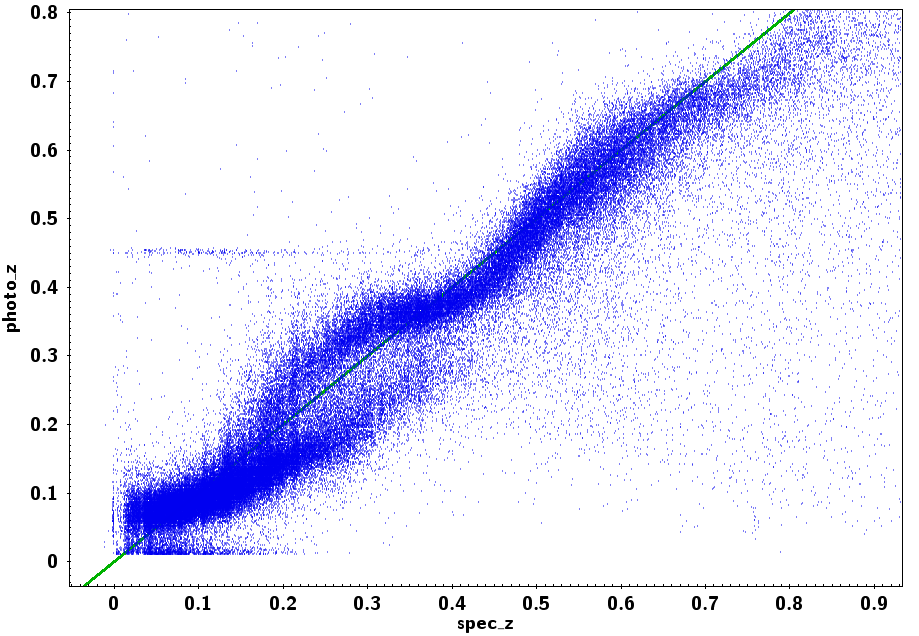
\includegraphics[width=5.7in]{Figures/photo_z_vs_spec_z.png}
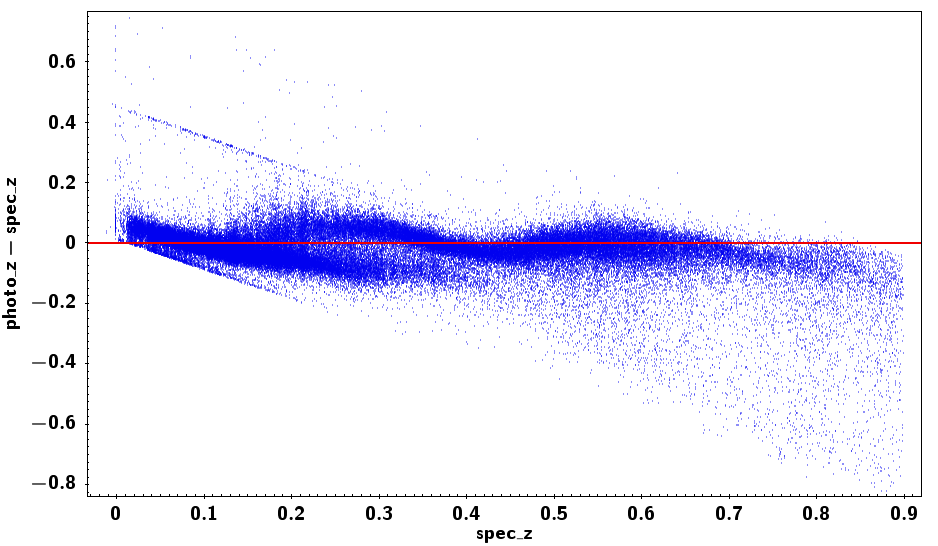
\includegraphics[width=5.7in]{Figures/photo_z_-_spec_z.png}
\caption{Comparison of z\_phot as calculated in EAZY to the z\_spec from the SDSS spectroscopic data. z\_phot vs z\_spec is plotted on top, another version of this plot, z\_phot - z\_spec vs z\_spec is plotted at the bottom. Despite several observable issues (especially around $z\approx 0.4$) the overall fit is satisfactory with the standard deviation as low as $\sigma=0.07$.}
\label{fig:photo_z}
\end{figure}

We provide the full list of EAZY parameters in \hyperref[sec:eazy]{Appendix}.

\subsection{Reliability of IR data}
It is well known that template errors in the rest-frame
near-IR can lead to degraded photo-z performance when
near-IR data is included (e.g., \citep{Brammer2008}).
\citep{2012AJ....144..188B} demonstrated acceptable z\_phot
performance with near-IR magnitudes included. They confirm that
the addition of UKIDSS photometry here does not improve the template z\_phot results, but also does not degrade them if photometry is appropriately weighted to
take template errors into account. 

We perform another run of EAZY with only optical photometry provided as input and compare the standard deviation of z\_spec vs z\_phot. As can be seen in Figure~\ref{fig:photo_z_nowise} near-IR filters do not significantly change the accuracy of the redshift estimation.

\begin{figure}[!ht]
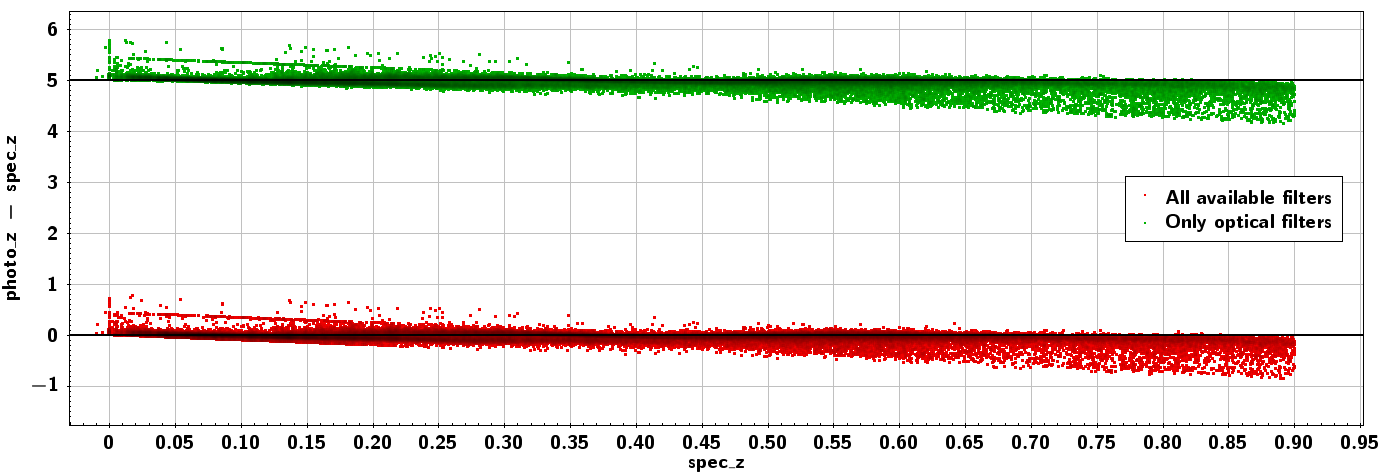
\includegraphics[width=5.7in]{Figures/photo_z_-_spec_z_nowise_wise.png}
\caption{Difference of z\_phot and z\_spec is plotted against z\_spec. Data obtained with all 7 or just 5 optical filters are plotted in red and green respectively.}
\label{fig:photo_z_nowise}
\end{figure}

\subsection{Stellar masses}

FAST (Fitting and Assessment of Synthetic Templates) \citep{2018ascl.soft03008K} is originally an IDL-based code that fits stellar population synthesis (SPS) \citep{2003MNRAS.344.1000B} templates to broadband photometry and (or) spectra. FAST is compatible with EAZY when fitting broadband photometry - it uses the photometric redshifts derived by that code as an input redshift. 
IDL (Interactive Data Language), is a programming language used for data analysis, it requires a license and is not installed on MU cluster machines so instead we use FAST++, a C++ version of FAST that can be found at \fnurl{GitHub}{https://github.com/cschreib/fastpp}. FAST++ code uses same input and output formats as FAST, is at least 4 times faster and apart from the single-threaded FAST is multithreading - it may use a number of concurrent threads (CPUs) that the program can use to speed up calculations, which is a significant advantage when working with a data sample as large as ours.
We tried several combinations of codes such as:\\
HyperZ for redshift estimation and FAST for stellar mass estimation;\\
HyperZ for redshift and stellar mass estimation;\\
EAZY for redshift estimation and HyperZ for mass estimation;\\
EAZY for redshift estimation and FAST for mass estimation;\\
and found the last option to be working best. So after we got photometric redshifts for all sources in our catalog with $SNR>5$ and non-zero flux in more than 4 filters, we supplied it along with the flux in $\mu$Jy to the FAST code. It takes around 12 hours CPU time to calculate masses for a set of $\approx60,000$ sources, so we used Lewis computational cluster again.
We present the mass histogram for four redshift bins of equal size on Figure~\ref{fig:hist_mass}. We see that galaxies in the lowest redshift bin are on average less massive then and tend to have stellar mass of $\sim10^{8.8}M_{sun}$, while galaxies in the higher redshifts peak around mass of $10^{10}M_{sun}$. This is can be explained by the incompleteness of our sample in high redshifts.

\begin{figure}[!ht]
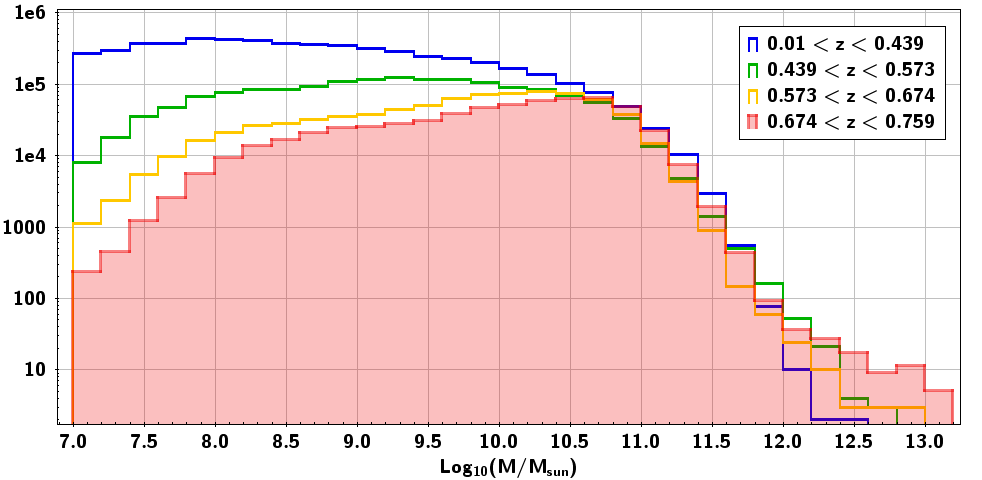
\includegraphics[width=5.7in]{Figures/histogram_all_stellar_mass_z_bins.png}
\caption{A histogram of masses for all four redshift bins. Galaxies in different bins end to peak at different masses, but galaxies in three high-redshift bins have the highest number of galaxies around similar stellar mass - $10^{10}$}
\label{fig:hist_mass}
\end{figure}

\section{Catalog post-procession}

At this point every source that has photometry in more than 4 filters has z\_phot and stellar mass assigned to it. But this data sample is not clean - there are stars, QSOs, also there are duplicate sources and sources with unreliable near-IR photometry due to the presence of nearby saturated sources. In the following subsections we explain our strategy of constructing the clean sample of galaxies.

\subsection{Star-galaxy separation}

Performing the classification of the sources is an important step in our project. Indeed, SED fitting codes may take photometric data of the star as a valid input and assign it some photometric redshift and stellar mass that does not have any physical significance ($\chi^{2}$ value of such objects is usually low, but this criteria is not enough to rejects stars). Such objects may severely alter the global density of objects and skew our results. In this section we attempt to find select galaxies alone from our sample and reject stars and other sources (mainly QSO) that are not a part of this project. Such selection is usually referred to as a "star-galaxy separation". One of the standard ways of performing this separation is via color-color diagram, on which stars and galaxies (hopefully) occupy different space on the graph. We tested several combination of bands in order to achieve best results (i.e. maximum possible number of galaxies rejected and minimal number of non-galaxies included in the sample) and found out that $"w1-i\; vs\; i-z"$ colors works best. As can be seen on (Figure~\ref{fig:sgs_color}), galaxies (blue), stars (red) and QSO (green) indeed occupy different space but with large overlapping regions, so the data set will neither be clean, nor complete. Another complication is that while we used r-band as a detection for the optical catalog and so all optical sources have consistent photometry in all 5 bands, some sources are shallow or undetected in w1 band. Such sources are assigned with w1\_{mag}=99 and thus occupy a low-left part of this diagram, outside of the reasonable regions. 

\begin{figure}[!ht]
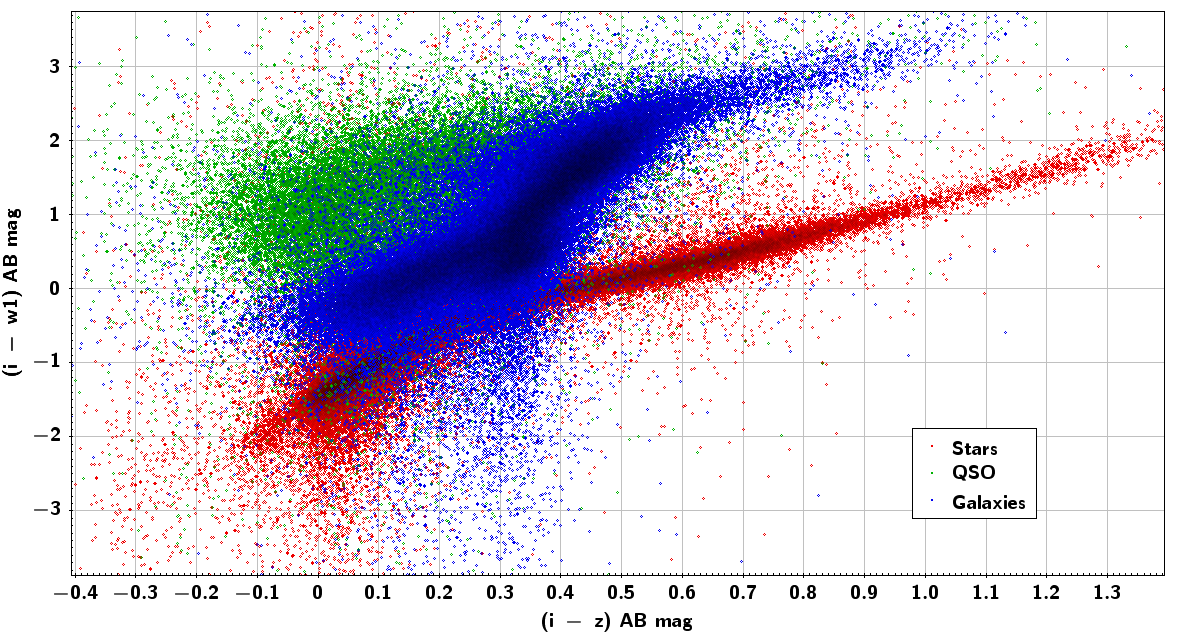
\includegraphics[width=5.7in]{Figures/star_galaxy_separation_color.png}
\caption{Color-color diagram for star-galaxy separation using $"w1-i\; vs\; i-z"$ colors.  Galaxies are plotted in blue, stars - in red and QSO in green. It is impossible to create a clean data sample using only colors as a selection criteria.}
\label{fig:sgs_color}
\end{figure}

Lack of IR data for some objects is a real disadvantage of the star-galaxy separation based on the color-color diagram, so we shall use another approach that is based on the "CLASS\_STAR" value - a stellarity index given by {\tt SExtractor}. Stellarity values near "0" indicate the object is likely a galaxy. If stellarity values near "1" that is a good indicator that an object is likely a star. To classify objects, {\tt SExtractor} uses a neural network which takes into account object attributes including FWHM. 
So the outline of our algorithm is as follows: the PSF functions that we built for every SDSS image will be used to measure FWHM of this image using {\tt irif/psfmeasure} task. Then this FWHM shall be supplied to the parameter file of SExtractor and another run of this code is performed in g-, r-, and i-bands (these bands are the most sensitive and generally have better FWHM over u- and z-bands).

Star-galaxy classification based on the CLASS\_STAR parameter that is measured in one band is about 95\% accurate (Figure~\ref{fig:sgs_hist}). We attempt to refine this result by finding the combination of selection criteria in three bands instead of just one.
We downloaded SDSS DR14 BOSS and SDSS spectrograph data in Stripe 82 region using \fnurl{CasJob Server}{https://skyserver.sdss.org/CasJobs/}. The size of this data set is 269,196 sources, each of which is assigned with spectroscopic class (can be GALAXY, QSO, or STAR) and extragalactic objects galaxies and QSO are also assigned with the z\_spec larger than 0. By matching this catalog to our main output catalog we got a set of data that contains 248,682 sources, which will serve as a training set for our star-galaxy separation.
We found the next criteria to perform the bet way:
$CLASS\_STAR\_r<0.2 \quad \&\& \quad CLASS\_STAR\_g<0.34 \quad \&\& \quad CLASS\_STAR\_i<0.70$\\
\begin{figure}[!ht]
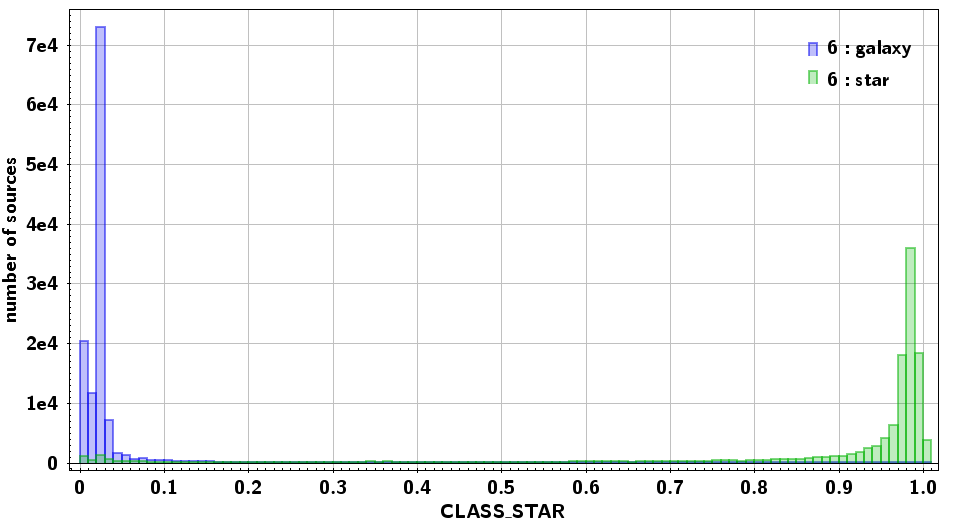
\includegraphics[width=5.7in]{Figures/histogram_class_star.png}
\caption{A histogram of the CLASS\_STAR values for r-band alone already shows efficiency of this method for star-galaxy separation. Galaxies and stars are selected from BOSS spectroscopic survey using parameter "CLASS". Galaxies are plotted in blue and tend to have smaller values of CLASS\_STAR, stars are plotted in green and on opposite - mostly have CLASS\_STAR value close to 1.}
\label{fig:sgs_hist}
\end{figure}

After this criteria has been applied to the data set we found that 3,874 galaxies (1.55\%) fall outside of the catalog and 4298 (1.73\%) stars and QSO are included into the sample (Figure~\ref{fig:sgs_hist}). We are satisfied with this result and perform the above criteria to the whole data set that decreases our total number of sources from 26,585,975 to 10,092,410 objects.

\begin{figure}[!ht]
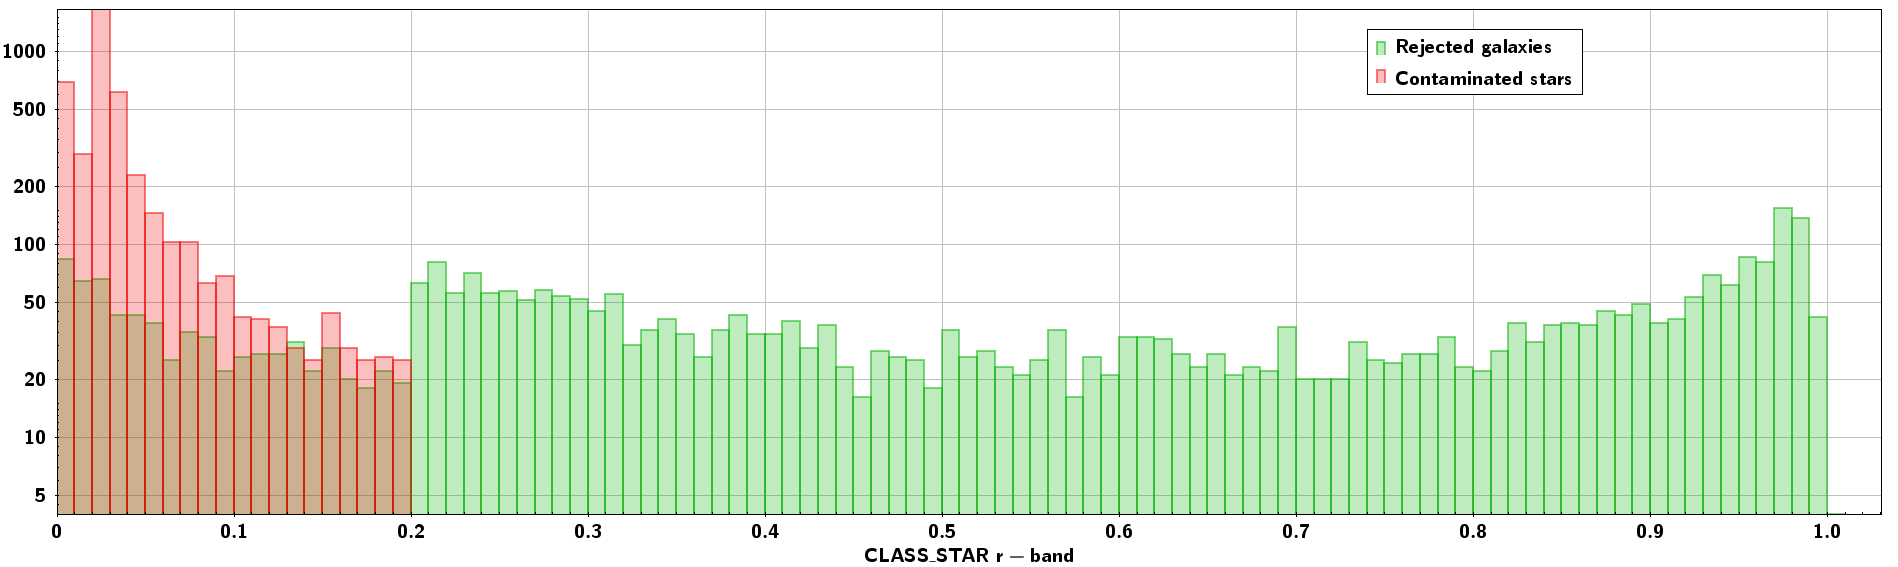
\includegraphics[width=5.7in]{Figures/histogram_class_star_contamination.png}
\caption{A histogram of the CLASS\_STAR values for galaxies from the control data sample that are rejected from our data sample due to very large CLASS\_STAR values (green). In red we plotted stars and QSO that are not excluded from our data sample - their CLASS\_STAR values are too small in all three optical bands that we used for star-galaxy separation.}
\label{fig:sgs_cont}
\end{figure}


\subsection{Sources treatment in overlapping regions and around bright stars}

Two adjacent SDSS images have overlapping regions - 25" wide for images in the same columns (i.e. their centers have the same Dec) and 28" wide for images in the neighbor columns (i.e. their centers have the same RA). Sources that appear in such regions are {\tt SExtracted} and {\tt TPHOTed} twice and have to be removed from the final catalog. We perform internal match on the catalog within all 80 unWISE frames and remove duplicate sources within 1.2 asec matching radius using {\tt STILTS} code. We verify that this radius is sufficient for removing majority of duplicate sources and also does not remove any non-duplicate sources in the main field that may have similar coordinates. This operation reduced the number of galaxies in our sample to 9,308,387 sources. An example of such duplicate sources is plotted with blue on Figure~\ref{fig:duplicate}

\begin{figure}[!ht]
\center{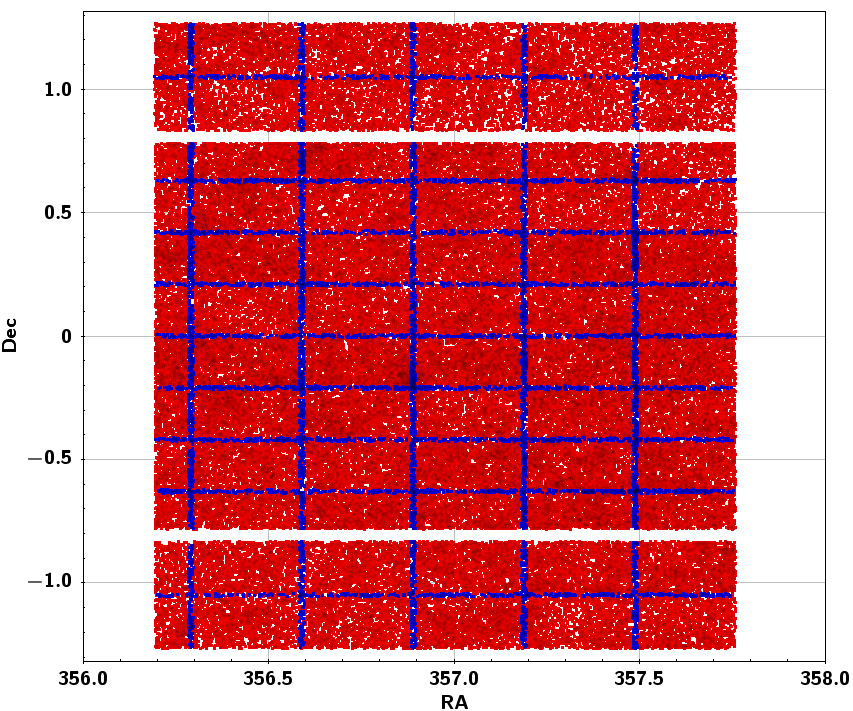
\includegraphics[height=4in]{Figures/duplicate_sources.png}}
\center{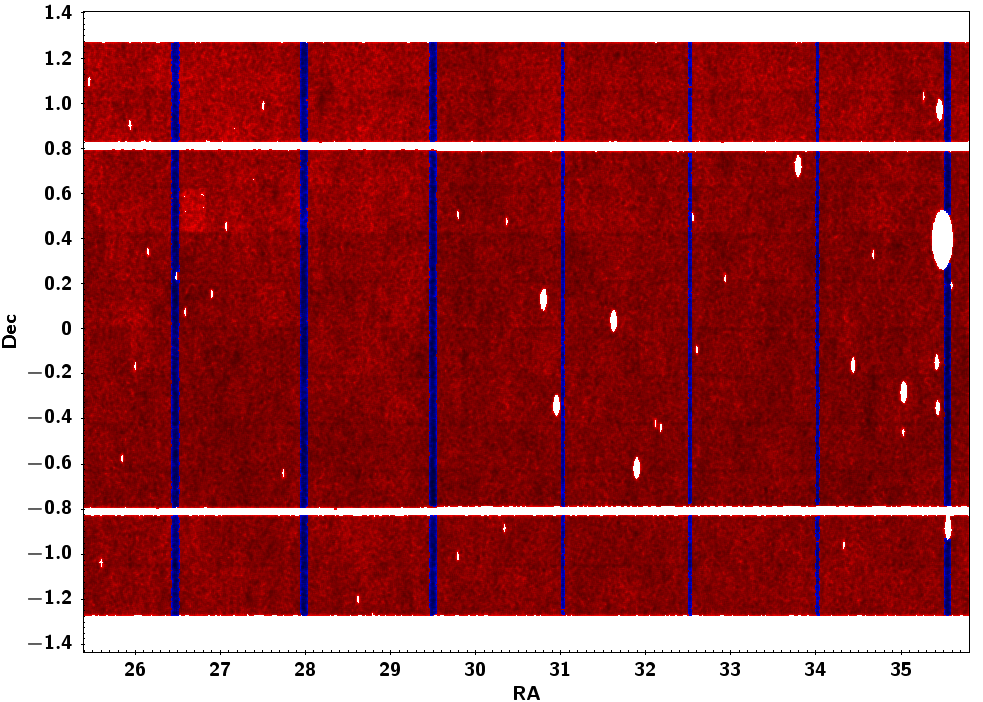
\includegraphics[height=4in]{Figures/duplicate_sources_wise.png}}
\caption{Duplicate sources (blue) are over-plotted with unique sources (red) in one unWISE frame that hosts 72 SDSS images (top image) and several adjacent unWISE frames (bottom image). Two white horizontal stripes between col07 and col02 (bottom) and coll11 and col06 (top) were also excluded from our project.}
\label{fig:duplicate}
\end{figure}

One unWISE frame consists of 3 unWISE images that have the same RA and are centered at Dec=$-1.6^{0}$, $0.0^{0}$ and $+1.5^{0}$. When we plotted SDSS images over unWISE frame, we noticed that each SDSS image from col07 and unWISE file that is centered at Dec=$+1.5^{0}$ overlap in a small region $\approx52.28$ square minutes. To process this small area in {\tt TPHOT} another 2,315 PSFs have to be constructed. We decided not to perform this very time-consuming operation and exclude this area, in total 5.55 $deg^{2}$ from our project. The same situation is with SDSS images from col02 and unWISE files centered at Dec=$-1.6^{0}$. Total area that was excluded from the project is 11.340 $deg^{2}$, it may be sen as two white horizontal stripes on Figure~\ref{fig:duplicate}

Objects that are extremely bright in near-IR present a number of problems to the photometry measurement by generating a host of artifacts. These artifacts include halos (low surface brightness emission extending well beyond the PSF), diffraction spikes, horizontal stripes and residual ghosts.
If not corrected, these artifacts will compromise the reliability of w1 and w2 photometry performed by TPHOT. To account for such artifacts the natural solution is to mask certain regions based on available catalogs. We used SAO star catalog \citep{Staff1966} and Bright IR Stars Compilation (BIRSC) [R. Tam and C. Xu - IPAC] as a base for the masking catalog. There are around 400 stars in both catalogs that fall within Stripe 82 footprint, but our visual inspection showed that some very bright objects (stars and galaxies) that severely alters results of {\tt TPHOT} are not in this list. We inspected all residual FITS images and added 300 more objects to the list that now consists of 706 objects. For stars from the catalog the masking area depends on the provided V-band magnitude and it was assigned manually based on the estimation of the halo for the added objects. Radii for masking are ranging from 50 to 500 arcsec. An example of such source with masking radius=100 asec is presented on Figure~\ref{fig:masking}. The overall masked area is 3.871 $deg^{2}$, which reduces the total sky area of the survey to 288.212 $deg^{2}$.

\begin{figure}[!ht]
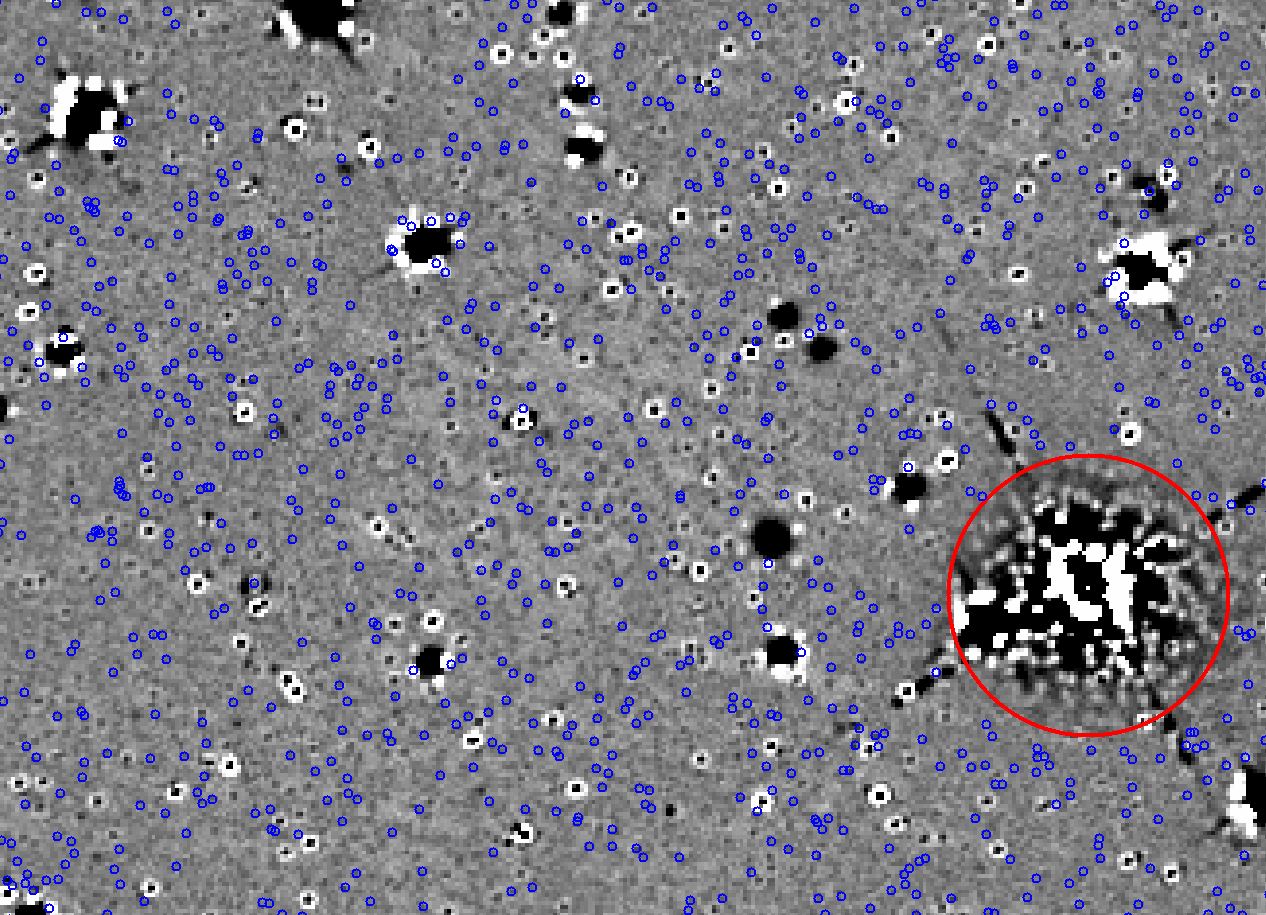
\includegraphics[width=5.7in]{Figures/CS_fits_region.png}
\caption{Residual image in w1 band with various regions plotted. All sources that were detected in r-band and supplied to TPHOT, but fall within the masked region (red) are excluded from the SED fitting. Blue circles 3 asec in radius show the position of objects, whose flux was subtracted from the unWISE image. Poorly subtracted objects (mostly stars) without blue circles around them were included into TPHOT input catalog, but later were excluded from ED fitting after star-galaxy separation}
\label{fig:masking}
\end{figure}

After rejection of such objects our catalog contains 9,061,068 objects and this is the final sample that we use as input to SED fitting codes that return photo$\_z$ and stellar mass that we use to build GSMD.
\chapter{Results}\label{CH_04}

\section{Binning in redshift}
Stellar mass density is calculated within some volume, so we bin our sample to four redshift intervals of the same comoving volume - $139,729,000 Mpc^{3}$. The size of the bin is chosen the way that we still have sufficient sources in the highest redshift bin that goes up to z=0.8 - even though our photometric redshifts span up to $z\approx~0.9$, the number sources at this redshift decreases significantly and this incompleteness leads to the severe underestimation of the number density. Information about binning is presented in Table~\ref{tab:redshift_bin}. Although it is tempting to create larger number of bin in order to see evolution of the stellar mass at "high-resolution", we remember that our redshift is determined based on photometry and thus is not reliable within better than $\Delta z\approx 0.1-0.15$ (also recall large scatter around $z\sim0.4$). So we decide to have four large bins in which errors in redshifts and associated stellar masses shall be averaged. Stellar mass is plotted against z\_phot in all four bins on Figure~\ref{fig:sm_z_dissect}.

\begin{figure}[!ht]
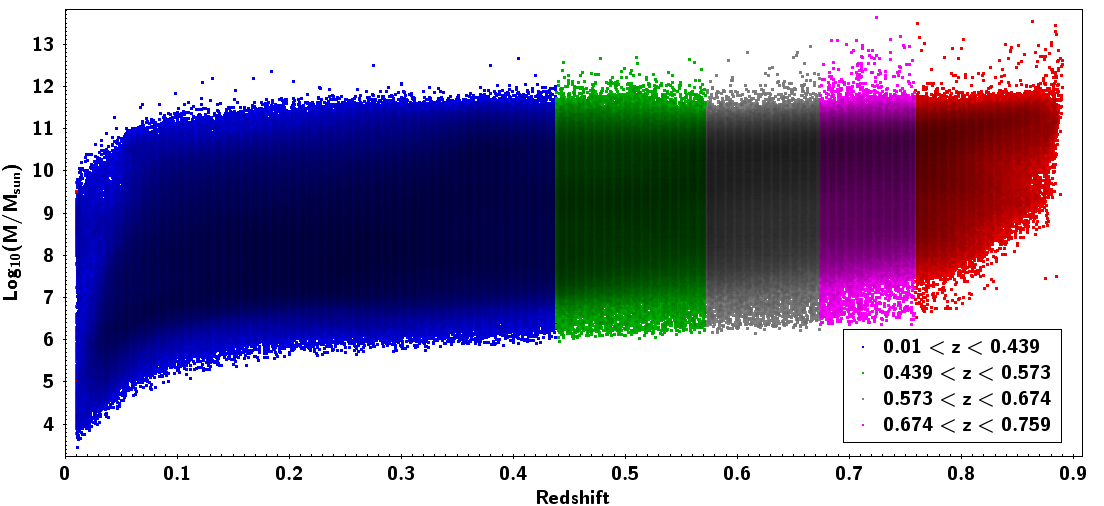
\includegraphics[width=6in]{Figures/mass_vs_photo_z_dissected.png}
\caption{Stellar mass density over photometric redshift. Four reddshift bins are plotted in different colors: z1 - blue, z2 - green, z3 - grey, z4 - magenta. Red sources at z$>$0.759 are not included into the sample due to their low number density.}
\label{fig:sm_z_dissect}
\end{figure}

\begin{table}[h!]
  \begin{center}
    \caption{Redshift binning of stellar mass}
    \begin{tabular}{l|l|l|l|l} % <-- Changed to S here.
     \textbf{\#} & \textbf{redshift} & \textbf{mean} & \textbf{\# of galaxies} & \textbf{fraction of galaxies}\\
     \textbf{} & \textbf{interval} & \textbf{redshift} & \textbf{per bin} & \textbf{per bin}\\
%      $\alpha$ & $\beta$ & $\gamma$ \\
      \hline
%      aperture [pix] & ?? & ?? & ?? & ?? & ??\\
      1 & 0.010$<z>$0.439 & 0.296 & 6,065,140 & 0.65\\
      2 & 0.439$<z<$0.573 & 0.506 & 1,588,509 & 0.17\\
      3 & 0.573$<z<$0.674 & 0.623 & 812,562  & 0.09\\
      4 & 0.674$<z<$0.759 & 0.716 & 585,009  & 0.06\\
    \end{tabular}
  \end{center}
  \label{tab:redshift_bin}
\end{table}

We sum up stellar mass of all galaxies in a bin and divide it by the bin volume to derive the stellar mass density per bin in units of $M_{\odot}/Mpc^{3}$. Stellar mass density is usually represented in a log scale. Also, in order to compare our results to other published data we scaled from a Chabrier IMF to a Salpeter IMF by multiplying the stellar masses by a factor of 1.64. Results are combined in Table~\ref{tab:smd} and will be published in \cite{Musin2018}.

\begin{table}[h!]
  \begin{center}
    \caption{Stellar mass density}
    \begin{tabular}{l|l|l|l|l|l|l} % <-- Changed to S here.
     \textbf{redshift} & \textbf{light-travel} & \textbf{total mass} & \text{total mass} & \textbf{$Log_{10}(\rho)$} & \textbf{$Log_{10}(\rho)$}\\
     \textbf{interval} & \textbf{time interval}          & \textbf{BC03} & \text{MA11} & \textbf{Chabrier IMF} & \textbf{Salpeter IMF}\\
	  \hline
       z & Gyr & $M_{\odot}$ & $Log_{10}(M_{\odot}/Mpc^{3})$ & $Log_{10}(M_{\odot}/Mpc^{3}$)\\
      \hline
      0.010$<z<$0.439 & 0.139-4.589 & $2.76\cdot 10^{16}$ & $2.72\cdot 10^{16}$ & 8.299 & 8.514\\
      0.439$<z<$0.573 & 4.589-5.537 & $1.89\cdot 10^{16}$ & $1.85\cdot 10^{16}$ & 8.077 & 8.292\\
      0.573$<z<$0.674 & 5.537-6.154 & $1.74\cdot 10^{16}$ & $1.52\cdot 10^{16}$ & 8.050 & 8.265\\
      0.674$<z<$0.759 & 6.154-6.619 & $1.74\cdot 10^{16}$ & $1.20\cdot 10^{16}$ & 8.089 & 8.304\\
    \end{tabular}
  \end{center}
  \label{tab:smd}
\end{table}

\begin{figure}[!ht]
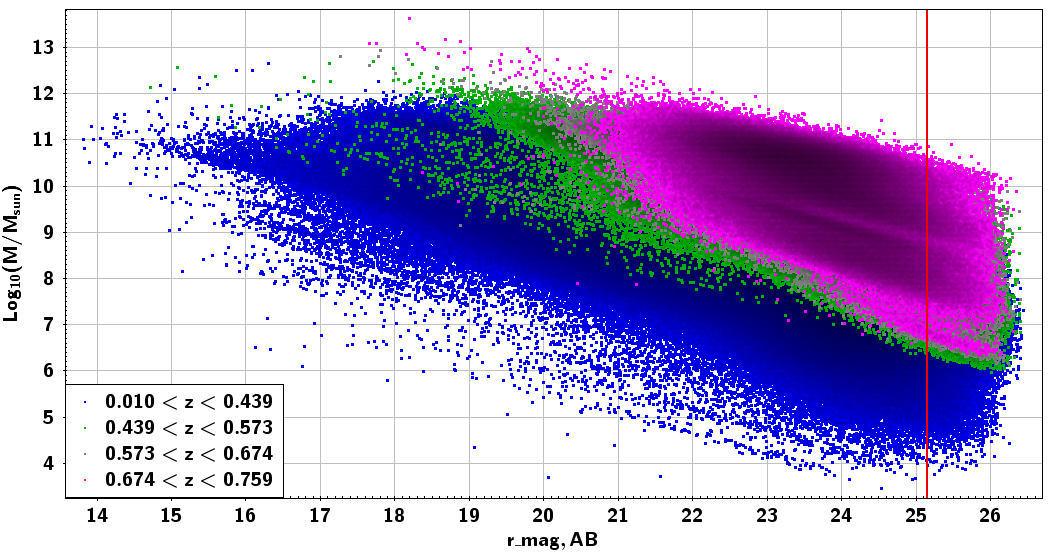
\includegraphics[width=6in]{Figures/mass_vs_r-mag.png}
\caption{Stellar masses are plotted over corresponding r-band magnitudes. Four redshift bins are plotted in different colors: z1 - blue, z2 - green, z3 - grey, z4 - magenta. Red vertical line denotes r-band $3\sigma$ detection limit.}
\label{fig:sm_mag_r}
\end{figure}

On the Figure~\ref{fig:sm_mag_r} we present stellar masses, binned to four redshifts as a function of r-band magnitude. Red vertical line shows the $3\sigma$ detection limit for the r-band. It does not necessarily mean that we should not trust masses beyond this limit as those sources may have reliable photometry in other bands, but it should at least be taken with caution.

\section{GSMD and comparison to the results of other groups}

In their review paper Madau \& Dickinson \citep{Madau2014} presented a compilation of recent measurements of SMD from different groups up to $z\approx 8$. They used all available data including wide field local SDSS based SMD. We predict that before any corrections our SMD should be somewhat close to reported results. We overplotted our derived SMD with red stars on top of the data presented in \citep{Madau2014}. As you may see on Figure~\ref{fig:gsmd_my} our points lie very close to some of the reported data, especially to \citep{2012A&A...545A..23B}, who used J,H and Ks filters to investigate the SMD in four CFHTLS deep fields.

Our reported mass density for the fourth redshift bin, 0.674$<z<$0.759 (8.089) is higher than that for the third one, 0.573$<z<$0.674 (8.050). It may not be a representation of any real processes, because even though generally stellar mass in a certain small volume can go down due to the end of the life cycle of massive stars, in general galaxies tend to increase their stellar mass in time. Interestingly, the same behavior is observed in the data of other groups, as can clearly be seen on Figure~\ref{fig:gsmd_my} in the region denoted by red rectangular. We interpret this "wiggle" in two ways - as a direct evidence of the incompleteness of our data sample or as a systematic overestimation of stellar masses in the highest redshift bin (some galaxies are assigned with stellar masses as high as $10^{13}M_{sun}$, which is not supported by any observations of galaxies at such redshifts. 

\begin{figure}[!ht]
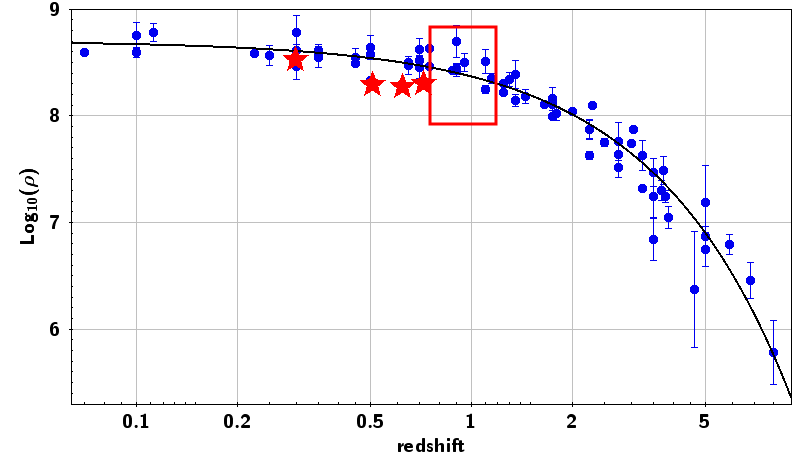
\includegraphics[width=6in]{Figures/md_plot_my_data_1.png}
\caption{Overplotted Figure 11 from Madau\&Dickinson 2014 with our SMD data points plotted as low-limit with with red stars. Data points inside the red rectangular demonstrate an odd "wiggle" upwards as if the SMD was higher in the earlier Universe. Black solid line is an approximation of the global stellar mass density obtained by integrating the best-fit instantaneous star-formation rate density}
\label{fig:gsmd_my}
\end{figure}

The problem of incompleteness appears in any survey, photometric or spectroscopic - low-mass galaxies at higher redshifts are too dim to be detected. Correction for incompleteness is beyond the scope of this thesis and we only outline here the possible approach. This incompleteness can be estimated based on a comparison to the much deeper small area surveys or based on the analytic correction that can be applied using the available data from Figure~\ref{fig:sm_z_dissect}.


\chapter{Summary and concluding remarks}\label{CH_summary}

\section{Conclusions}

In this thesis we investigated the evolution of galaxies by studying the growth of stellar mass and stellar mass density in time in the last 6 Gyr. We combined the datasets from two very large surveys and built the largest catalog of galaxies to date that has consistent fluxes in 5 optical (SDSS) and 2 near-IR (WISE) bands and contains over 9 million galaxies. This consistency has been achieved in two ways:\\ 
- in optical all bands were convolved with the PSF of the band with the worst FWHM, namely u-band. We did this by constructing PSF functions for each individual SDSS image. Then, using r\_matched\_u band as a detection image we extracted fluxes of the sources sources in SDSS Stripe 82 field.\\
- in near-IR the angular resolution is $\approx 6$ times worse than in optical, so we applied "template-fitting" technique in which we use the high-resolution image to define the morphological template of the galaxy in question, and de-convolve its light profile in the low-resolution image.

This approach allows us to perform SED measurements in the restframe near-IR regime, which is important for the correct estimation of the dust extinction and contribution of the low-mass stars, which may be outshone by brighter stars in optical, and thus are accountant, but contribute significantly to the total stellar mass of the galaxy. We derive photometric redshifts and stellar masses for all the 9 million galaxies that span at $z=0$-0.8 and calculated stellar mass density over four redshift bins. Our SMD (we call it low-limits, since we did not correct for incompleteness of low-mass galaxies in the higher redshift bins) are generally close to the previously reported results, but with a much larger statistics over significant portion of the sky. Our result contribute to the GSMD and shall be used in future to provide constraints on any models of the galaxy evolution at high redshifts.

\section{Future work}

In 2010, after the depletion of coolant in the WISE telescope, w3 and w4 became unusable. Nevertheless, WISE continued surveying the sky through January 2011 in w1 and w2 as they are less affected by the rising temperature of the sensor, including a portion of the mission referred to as NEOWISE \citep{2011ApJ...731...53M}. WISE was placed in hibernation in February 2011, and was later reactivated in October 2013 and continued surveying the sky in w1 and w2. This survey is referred to as NEOWISE-Reactivation (NEOWISER) and continued until 2017. NEOWISER images are of very nearly the same high quality as those of the pre-hibernation WISE mission and it was quickly appreciated by the astronomical community. \citep{1538-3881-154-4-161} created a set of co-add images following procedures in D14 for all available data in bands w1 and w2. This not only made the images more sensitive (by 0.38 magnitudes in both bands), but significantly reduce the noise and allowed to clean out transient and spurious sources. That is very important to us because as you may see in the Figure~\ref{fig:sm_w1-mag} lots (58\%) of the sources are below the detection limit. We still supply such sources to TPHOT for the reasons to be explained in the next subsection, but their near-IR magnitudes are untrustworthy. New data from \citep{1538-3881-154-4-161} will add 5\% more sources above the detection limit and make stellar mass estimation more robust.

\begin{figure}[!ht]
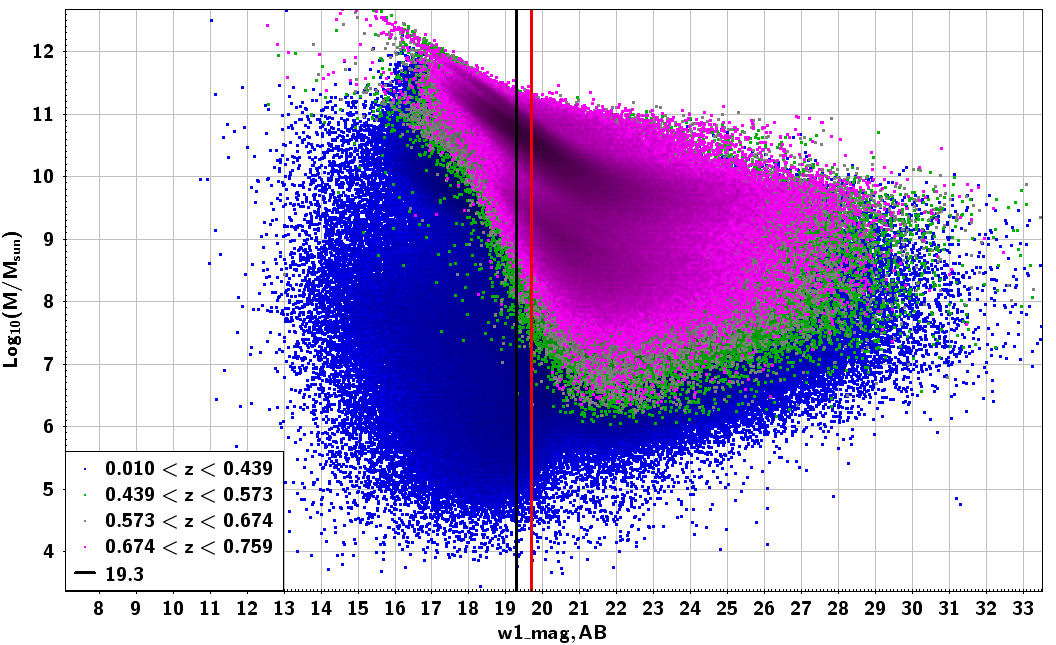
\includegraphics[width=6in]{Figures/mass_vs_w1-mag.png}
\caption{Stellar masses are plotted over corresponding w1-band magnitudes. Four redshift bins are plotted in different colors: z1 - blue, z2 - green, z3 - grey, z4 - magenta. Black vertical line denotes the $5\sigma$ detection limit for unWISE, red vertical image - analogous detection limit for the stacked WISE and NEOWISER data}
\label{fig:sm_w1-mag}
\end{figure}

In order to use these images we need to construct 240 new PSFs per band (480 in total) convolve them to already existing r\_matched\_u PSFs and re-run the TPHOT over entire Stripe 82 region. Such run, though time-consuming, will not only significantly increase the precision of the near-IR photometry, but also increase the total number of sources. In deeper near-IR images more sources will have non-zero fluxes - so sources that now have photometric fluxes in less then 4 bands and are currently not supplied for SED fitting will be included in the stellar mass density estimation. 

\subsection{Optical dropouts in WISE}
Residuals in w1 and w2 that are produced by TPHOT reveal a mysterious population of objects with SNR$>5$ in both bands. The fact that they were not "cleaned out" by TPHOT suggests that they are invisible in optical and our inspection of SDSS images proves this. We call them "WISE optical dropouts" (WoDrops) and investigating their nature is a follow-up for this project, though some preparatory work has been already done.\\
- Using the latter WISE observations in w1 and w2 during "3-Band Cryo" and "NEOWISE" programs, we verified that these objects cannot be transients.\\
- Their colors ($w1-z>4.8$ AB mag) cannot be explained by Galactic brown dwarfs.\\
- WoDrops cannot be a high-redshift ($z>7$) objects due to their large number density (\~176/square degree) - that contradicts to current observations of the population of the most luminous quasars.\\
An example of such WoDrop is presented in Figure~\ref{fig:wodrop_sdss}

\begin{figure}[!ht]
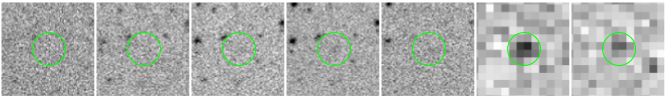
\includegraphics[width=6in]{Figures/wodrop_sdss_w1w2.png}
\caption{An example of WoDrop. Shown from left to right are the $ugriz$ and unWISE w1 and w2 images. The images are 33"x33" in size, and the green circles indicate the location of the WoDrop. For this particular example is SNR = 8 and 5.4 for bands w1 and w2 respectively.}
\label{fig:wodrop_sdss}
\end{figure}

The only reasonable explanation is that these objects may be a low-redshift (z$\sim0.5$) old, massive but passive galaxies that resemble in colors Spitzer IRAC-selected Extremely Red Objects (IERO) \citep{Yan2004}. If this is really the case then our low-$z$ stellar mass density may be underestimated. In order to better understand the nature of such objects we need data in the near-IR regime, namely filters J, H and Ks - they lie in between optical filters $ugriz$ and w1, w2 bands. Figure~\ref{fig:wodrop_sed} shows an example of the SED fitting for one of the WoDrops. w1 and w2 photometry is shown in magenta, non-detection in optical bands is plotted with upper-limits in grey and possible photometry for J, H and Ks bands is in blue.

\begin{figure}[!ht]
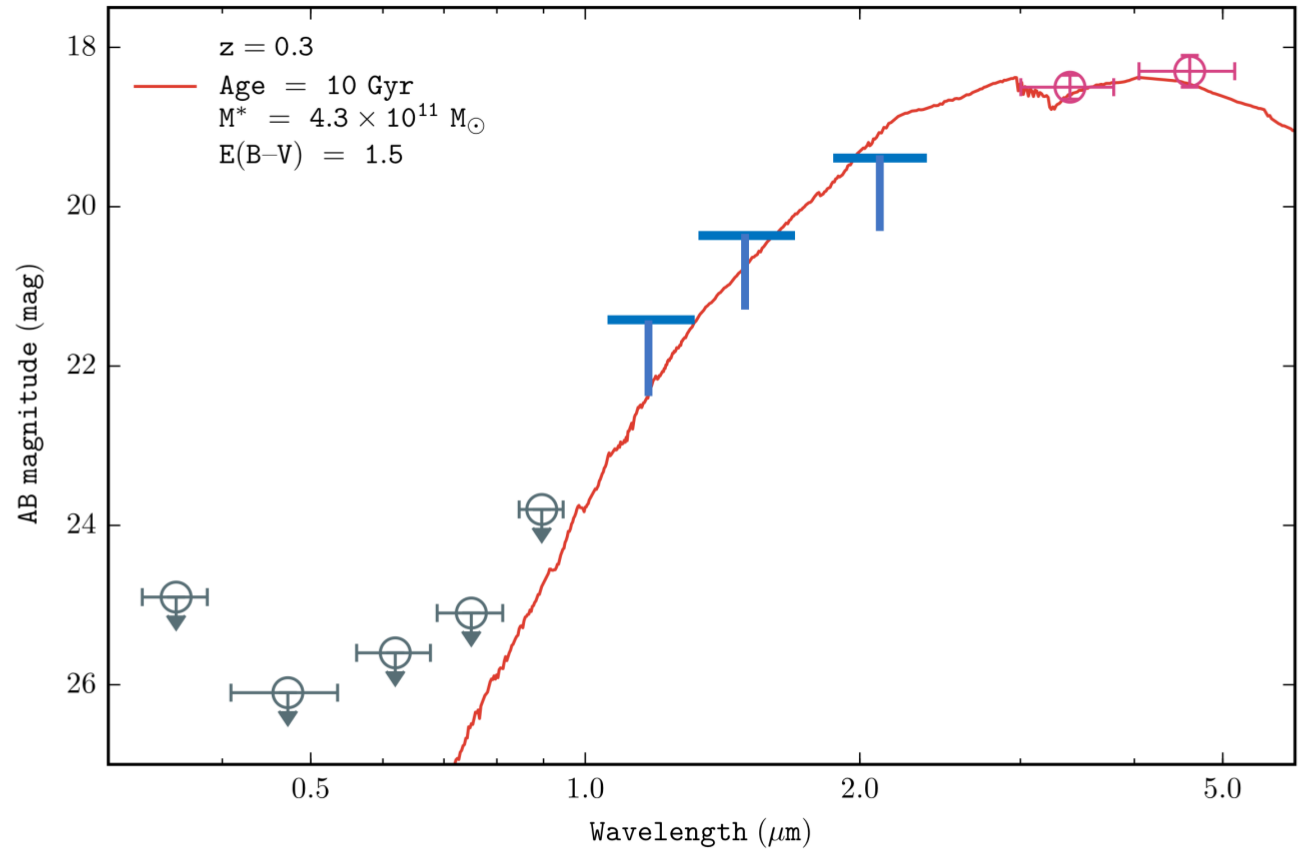
\includegraphics[width=6in]{Figures/wodrop_sed.png}
\caption{Illustration of the probable explanation to the nature of WoDrops. The photometry of this object in w1 and w2 are indicated by the two magenta points, and its non-detection in the Stripe 82 $ugriz$ images is indicated by the $2\sigma$ upper limits shown in grey.}
\label{fig:wodrop_sed}
\end{figure}

To date only quarter of the Stripe 82 footprint has been searched for the presence of WoDrops. We expect to find $\approx52,800$ dropouts. Creating the full set of WoDrops requires careful visual inspection of thousands of images, is extremely time-consuming but shall be completed in the nearest future.

We used several opportunities to add complementary photometric data to catalog. A fraction of sources is detected in IRAC SHELA - a $24 deg^{2}$ survey at 3.6 and 4.5 microns \citep{Papovich2016}. This survey is complete to 22.0 AB limiting magnitude but covers less than 10\% of Stripe 82. 

Five objects were observed with WIYN High Resolution Infrared Camera (WHIRC) \citep{Smee2011a}. Figure~\ref{fig:wodrop_whirc} shows that results are contradictory - after 3 hours of the total integration time per source only one source has detection in H and Ks, but not in J. All other sources are undetected. This non-detection is even a more interesting result as it may be a signal of detecting a new population of objects. 

\begin{figure}[!ht]
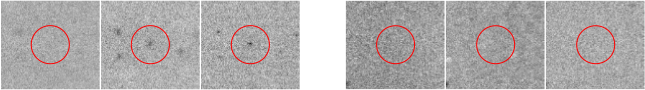
\includegraphics[width=6in]{Figures/wodrop_whirc.png}
\caption{An example of two WoDrops that have been observed by near-IR imager WHIRC instrument at WIYN telescope. All images are 33"x33" in size, and the red circles indicate the location of the WoDrop. The nominal on-source exposures are 31 min, 43 min and 1.1 hrs in Ks, but as can be seen, one WoDrop is only detected in H and Ks band, while the second one is not detected (as well as other three WoDrops that were observed in this run)}
\label{fig:wodrop_whirc}
\end{figure}

To further investigate the nature of these objects, an observing proposal was submitted to the Large Binocular Telescope (LBT) telescope to observe another 20 WoDrops (LBTO Reference: TS-2018B-006, PI - Haojing Yan). This 8m class telescope is equipped with LUCI (originally LUCIFER) - Large Binocular Telescope Near-infrared Spectroscopic Utility with Camera and Integral Field Unit for Extragalactic Research. LUCI operates in the 0.9 - 2.5 micron spectral range and provides imaging and spectroscopic capabilities in seeing- and diffraction limited modes.
\newpage
\phantomsection\addcontentsline{toc}{chapter}{APPENDIX}
\appendix

\chapter{Parameters for applied codes}\label{AP_01}

\section{SExtractor parameters for x$\_$matched$\_$u catalogs}
\label{sec:sex}

\begin{tt}
DETECT$\_$TYPE      CCD            $\#$ CCD (linear) or PHOTO (with gamma correction)\\
DETECT$\_$MINAREA   3              $\#$ minimum number of pixels above threshold\\
THRESH$\_$TYPE      RELATIVE       $\#$ threshold type: RELATIVE (in sigmas)\\
                                $\#$ or ABSOLUTE (in ADUs)\\
DETECT$\_$THRESH    2.5            $\#$ <sigmas> or <threshold>,<ZP> in mag.arcsec-2\\
ANALYSIS$\_$THRESH  2.5            $\#$ <sigmas> or <threshold>,<ZP> in mag.arcsec-2\\
FILTER           Y              $\#$ apply filter for detection (Y or N)?\\
FILTER$\_$NAME      gauss$\_$2.0$\_$5x5.conv   $\#$ name of the file containing the filter\\
FILTER$\_$THRESH                   $\#$ Threshold[s] for retina filtering\\
DEBLEND$\_$NTHRESH  32             $\#$ Number of deblending sub-thresholds\\
DEBLEND$\_$MINCONT  0.005          $\#$ Minimum contrast parameter for deblending\\
CLEAN            Y              $\#$ Clean spurious detections? (Y or N)?\\
CLEAN$\_$PARAM      1.0            $\#$ Cleaning efficiency\\
MASK$\_$TYPE        CORRECT        $\#$ type of detection MASKing: can be one of\\
                                $\#$ NONE, BLANK or CORRECT\\
WEIGHT$\_$TYPE      MAP$\_$WEIGHT,MAP$\_$WEIGHT           $\#$ type of WEIGHTing: NONE, BACKGROUND,\\
                                $\#$ MAP$\_$RMS, MAP$\_$VAR or MAP$\_$WEIGHT\\
WEIGHT$\_$GAIN      N,N              $\#$ modulate gain (E/ADU) with weights? (Y/N)\\
WEIGHT$\_$THRESH                   $\#$ weight threshold[s] for bad pixels\\
FLAG$\_$IMAGE       flag.fits      $\#$ filename for an input FLAG-image\\
FLAG$\_$TYPE        OR             $\#$ flag pixel combination: OR, AND, MIN, MAX\\
                                $\#$ or MOST\\
PHOT$\_$APERTURES   9.0            $\#$ MAG$\_$APER aperture diameter(s) in pixels\\
PHOT$\_$AUTOPARAMS  2.5, 3.5       $\#$ MAG$\_$AUTO parameters: <Kron$\_$fact>,<min$\_$radius>\\
PHOT$\_$PETROPARAMS 2.0, 3.5       $\#$ MAG$\_$PETRO parameters: <Petrosian$\_$fact>,\\
                                $\#$ <min$\_$radius>\\
PHOT$\_$AUTOAPERS   0.0,0.0        $\#$ <estimation>,<measurement> minimum apertures\\
                                $\#$ for MAG$\_$AUTO and MAG$\_$PETRO\\
PHOT$\_$FLUXFRAC    0.5            $\#$ flux fraction[s] used for FLUX$\_$RADIUS\\
SATUR$\_$LEVEL      25000.0        $\#$ level (in ADUs) at which arises saturation\\
SATUR$\_$KEY        SATURATE       $\#$ keyword for saturation level (in ADUs)\\
MAG$\_$ZEROPOINT    00.0\\
MAG$\_$GAMMA        4.0            $\#$ gamma of emulsion (for photographic scans)\\
GAIN             0.0            $\#$ detector gain in e-/ADU\\
GAIN$\_$KEY         GAIN           $\#$ keyword for detector gain in e-/ADU\\
PIXEL$\_$SCALE      0.396            $\#$ size of pixel in arcsec (0=use FITS WCS info)\\
SEEING$\_$FWHM      1.5            $\#$ stellar FWHM in arcsec\\
STARNNW$\_$NAME     default.nnw    $\#$ Neural-Network$\_$Weight table filename\\
BACK$\_$TYPE        AUTO           $\#$ AUTO or MANUAL\\
BACK$\_$VALUE       0.0            $\#$ Default background value in MANUAL mode\\
BACK$\_$SIZE        8\\
BACK$\_$FILTERSIZE  3              $\#$ Background filter: <size> or <width>,<height>\\
BACKPHOTO$\_$TYPE   GLOBAL         $\#$ can be GLOBAL or LOCAL\\
BACKPHOTO$\_$THICK  24             $\#$ thickness of the background LOCAL annulus\\
BACK$\_$FILTTHRESH  0.0            $\#$ Threshold above which the background-\\
                                $\#$ map filter operates\\
  \end{tt}


\section{TPHOT parameters}
\label{sec:tphot}
\begin{tt}

order standard $\#$1st pass\\
order standard2 $\#$2nd pass\\
usereal         True\\
usemodels       False\\
useunresolved   False\\
normalize       true\\
subbckg         True\\
savecut         false\\
cutoutdir       cutouts\\
cutoutcat       cutouts$\/$cutouts.cat\\
modelscat       models$\/$models.cat\\
modelsdir       models\\
culling         false\\
errtype         wht\\
rmsconstant     1\\
relscale        7\\
FFTconv         true\\
multikernels    false\\
mkext           false\\
kernellookup    ch1$\_$dancecard.txt\\
templatedir     templates\\
templatecat     templates$\/$templates.cat\\
fitpars          tpipe$\_$tphot.param1\\
tphotcat         lores$\_$tphot.cat$\_$pass1\\
tphotcell        lores$\_$tphot.cell$\_$pass1\\
tphotcovar       lores$\_$tphot.covar$\_$pass1\\
fitting         single\\
cellmask        true\\
maskfloor       1e-9\\
fitbackground   false\\
fit$\_$loc$\_$bkgd    0\\
writecovar      true\\
threshold       0.0\\
linsyssolver    lu\\
clip            true\\
rmscheck        0\\
modelfile       lores$\_$collage$\_$pass1.fits\\
dzonesize       5\\
maxshift        0.5\\
ddiagfile       ddiags.txt\\
dlogfile        dlog.txt\\
dancefft        true\\
nneighinterp    0\\
\end{tt}

\section{EAZY parameters}
\label{sec:eazy}
\begin{tt}
FILTER$\_$FORMAT        1                  $\#$ Format of FILTERS$\_$RES file -- 0: energy-  1: photon-counting detector\\
SMOOTH$\_$FILTERS       y                  $\#$ Smooth filter curves with Gaussian\\
SMOOTH$\_$SIGMA         100.               $\#$ Gaussian sigma (in Angstroms) to smooth filters\\
TEMPLATES$\_$FILE       eazy$\_$v1.3.spectra.param $\#$ Template definition file\\
TEMPLATE$\_$COMBOS      a                  $\#$ Template combination \\
NMF$\_$TOLERANCE        1.e-4              $\#$ Tolerance for non-negative combinations (TEMPLATE$\_$COMBOS=a)\\
TEMP$\_$ERR$\_$A2          1.00               $\#$ Template error amplitude\\
SYS$\_$ERR              0.00               $\#$ Systematic flux error\\
APPLY$\_$IGM            y                  $\#$ Apply Madau 1995 IGM absorption\\
DUMP$\_$TEMPLATE$\_$CACHE  n                  $\#$ Write binary template cache\\
USE$\_$TEMPLATE$\_$CACHE   n                  $\#$ Load in template cache\\
CACHE$\_$FILE           tempfilt.dat       $\#$ Template cache file (in OUTPUT$\_$DIRECTORY)\\
NOT$\_$OBS$\_$THRESHOLD    -90                $\#$ Ignore flux point if <NOT$\_$OBS$\_$THRESH\\
N$\_$MIN$\_$COLORS         4                  $\#$ Require N$\_$MIN$\_$COLORS to fit\\
CHI2$\_$SCALE           1.0                $\#$ Scale ML Chi-squared values to improve confidence intervals\\
APPLY$\_$PRIOR          n                  $\#$ Apply apparent magnitude prior\\
PRIOR$\_$ABZP           23.9               $\#$ AB zeropoint of fluxes in catalog.!\\
FIX$\_$ZSPEC            n                  $\#$ Fix redshift to catalog zspec\\
Z$\_$MIN                0.01               $\#$ Minimum redshift\\
Z$\_$MAX                0.9                $\#$ Maximum redshift\\
Z$\_$STEP               0.01               $\#$ Redshift step size\\
Z$\_$STEP$\_$TYPE          1                  $\#$  0 = ZSTEP, 1 = Z$\_$STEP*(1+z)\\
GET$\_$ZP$\_$OFFSETS       n                  $\#$ Look for zphot.zeropoint file and compute zeropoint offsets\\
H0                   70.0               $\#$  Hubble constant\\
OMEGA$\_$M              0.3                $\#$ Omega matter\\
OMEGA$\_$L              0.7                $\#$ Omega lambda\\
\end{tt}

\section{FAST parameters}
\label{sec:fast}
\begin{tt}SAVE$\_$SIM           = 0             $\#$ 0 / 1			\\
SFR$\_$AVG            = 0             $\#$ 0, 100 Myr, 300 Myr etc\\		
INTRINSIC$\_$BEST$\_$FIT = 0             $\#$ 0 / 1				\\
BEST$\_$SFHS          = 0             $\#$ 0 / 1\\
SFH$\_$OUTPUT$\_$STEP    = 10            $\#$ 10 Myr, 100 Myr etc\\
SFH$\_$OUTPUT         = 'sfr'         $\#$ 'sfr' or 'mass'\\
REST$\_$MAG           = []            $\#$ [140,142,161] for UVJ colors\\
CONTINUUM$\_$INDICES  = ''\\
OUTPUT$\_$COLUMNS     = []            $\#$ ['id','Av','lmass','lsfr', ...]\\
LIBRARY             = 'bc03'         $\#$ 'bc03' / 'ma05' / 'co11'\\
RESOLUTION          = 'hr'           $\#$ 'pr' / 'lr' / 'hr'\\
IMF                 = 'ch'           $\#$ 'ch' / 'sa' / 'kr'\\
SFH                 = 'exp'          $\#$ 'exp' / 'del' / 'tru'\\
DUST$\_$LAW            = 'calzetti'     $\#$ 'calzetti' / 'mw' / 'kc' / 'noll'\\
LOG$\_$TAU$\_$MIN    = 6.5            $\#$ log [yr]\\
LOG$\_$TAU$\_$MAX    = 11.0           $\#$ log [yr]\\
LOG$\_$TAU$\_$STEP   = 0.1            $\#$ log [yr], min 0.1\\
LOG$\_$AGE$\_$MIN    = 6.0            $\#$ log [yr]\\
LOG$\_$AGE$\_$MAX    = 10.2           $\#$ log [yr]\\
LOG$\_$AGE$\_$STEP   = 0.1            $\#$ log [yr]\\
NO$\_$MAX$\_$AGE     = 0              $\#$ 0 / 1\\
Z$\_$MIN          = 0.01           $\#$ Cannot be 0.0\\
Z$\_$MAX          = 0.90\\
Z$\_$STEP         = 0.005\\
Z$\_$STEP$\_$TYPE    = 0              $\#$ 0: Z$\_$STEP, 1: Z$\_$STEP*(1+z)\\
A$\_$V$\_$MIN        = 0.             $\#$ [mag]\\
A$\_$V$\_$MAX        = 1.6            $\#$ [mag]\\
A$\_$V$\_$STEP       = 0.05           $\#$ [mag]\\
METAL          = [0.02]         $\#$ [0.0096,0.019,0.03]\\
NO$\_$CACHE       = 0              $\#$ 0 / 1\\
H0             = 70.0               $\#$ Hubble constant\\
OMEGA$\_$M        = 0.3                $\#$ Omega matter\\
OMEGA$\_$L        = 0.7                $\#$ Omega lambda\\
SAVE$\_$CHI$\_$GRID  = 0          $\#$ 0 / 1\\
\end{tt}
\newpage
\phantomsection\addcontentsline{toc}{chapter}{BIBLIOGRAPHY}
\bibliographystyle{plainnat}
%\bibliographystyle{unsrt}
\bibliography{ThesisMaster}


%\input{Fucknowledge}
\newpage
\phantomsection\addcontentsline{toc}{chapter}{VITA}

\centerline{\bf \large VITA}
\vspace{10mm} % Edit everything below with your acknowledging text.



Marat Musin was born on May 22, 1986 in Moscow, Russia, to the parents of Damir and Dina Musin. He graduated from Moscow Power Engineering Institute, Russia, in February, 2009 with an Engineering degree in Industrial Electronics. He worked as an Engineer at Ruselprom Inc until June, 2011. In August, 2011 he entered the graduate program in Physics and Astronomy at the University of Missouri-Columbia under supervision of Professor Haojing Yan and defended his thesis in May, 2018.


\end{document}
